\chapter{Concept for an Exergame for Elderly}
\label{chap:concept}
This chapter is about the second and third step in the cycle of user centered design, specifying requirements and producing design solutions, see Figure \ref{userdesign}. Based on findings from workshop 1, knowledge about elderly and exercise, and studies done on elderly and video games, we have created system requirements and designed a video game concept for an exergame for elderly. The exergame focus on including movement and exercise in real-life and well-known activities, in an entertaining and motivating way. We will present the requirements this video concept is built upon, before we describe our exergame concept in more detail. This will include games and challenges, the exercises used, goals, obstacles, and how to achieve points. In addition to the exergame concept, we have also, based on a course in \ac{hci} at NTNU, and guidelines for developing interfaces for elderly, designed a menu for the exergame. 

The exergame concept will be presented based on theory on designing video games, as discussed in Chapter \ref{chap:vg}, and can serve as a part of a design document, according to what is described in Section \ref{sec:designphase}. \cite{gamedesign} states that technical details should not be included in this document, while \cite{understandingvg} join them. The technical details are not the main focus in this thesis. However, we have included a brief description of some non-functional requirements, and therefore follows the way \cite{understandingvg} describes a design document. We acknowledge that not all the elements that should be included in a design document are present in this chapter, due to the scope of our thesis.

When creating the exergame concept, we have highly focused on the intended user group. The concept is based upon the requirement specification. In addition to this, expressed thoughts and opinions from the informants during workshop 1 are emphasised. The figures in this chapter are prototypes presenting what the exergame concept will look like. We will use these prototypes to present the concept idea and design for elderly in a second workshop, and we have therefore focused on making prototypes that gives the users a realistic impression of the final result. The prototypes are medium-fidelity prototypes, made with software tools as PowerPoint and Photoshop. We have chosen to use these software tools, as they are familiar to us, and therefore did not require spending time learning new tools. Because this concept is in an early stage of a development process, we did not want to spend too much time and effort making prototypes. The prototypes presented in this chapter will be in English, to be in accordance with the language this master thesis is written in. The original prototypes are in Norwegian and can be found in Appendix C and D. 

We will start by presenting the system requirements for the exergame concept in Section \ref{sec:req}, before we continue with describing our exergame concept with its story and included elements. Various scenarios will be presented with the use of medium-fidelity prototypes. This will be presented in \ref{sec:outinthenature}. Functional design, presented in Section \ref{sec:functionaldesign}, will give a concrete representation of the exergame concept. Design and description of the menu for the exergame concept are shown in \ref{sec:menu}. This chapter can be serve as a guide for a developer team that wants to understand and design an exergame. Beside those requirements that will be presented in this chapter, there exist other aspects to consider when developing an exergame for elderly. These aspects goes beyond our area of competence, and are therefore not the focus in our master thesis. However, they will be presented in Section \ref{sec:misc}.

\section{Requirements}
\label{sec:req}
We have set up a list of requirements for the exergame concept, which specifies what our system shall do, and which constraints the system shall hold. The requirements has been developed with foundation in video game theory, guidelines for usability, and findings from workshop 1. We have written requirements for the exergame concept according to what we have presented about requirement specification in Section \ref{sec:fourpillarsofdesign}, and they are therefore divided into functional and non-functional requirements. In the exergame concept we have mostly focused on the functional requirements, and interface requirements, which is a subsection of non-functional requirements. We will support our requirement specification by referring to relevant references, findings (referred to as fw1), and guidelines listed in Section \ref{sec:summaryguidelines} and Section \ref{subsec:golden}.

\subsection{Functional Requirements}
The functional requirements in Table \ref{tab:func1} and \ref{tab:func2} present which services and functionality the exergame concept shall offer.

\begin{table} [H]
\centering
\begin{tabular}{|>{\raggedright}p{0,7cm}|p{8,3cm}|p{2cm}|}
\hline
1.1 & The system shall be an exergame that emphasises exercise and physical movement. & ref: \cite{project} \\ \hline
1.2 & The system shall have a fun and entertaining story with focus on game play.  & ref: \cite{project} \cite{zyda2005visual} \\ \hline
1.3 & Exercise shall be subordinate to the story.  & ref:\cite{zyda2005visual} \\ \hline
1.4 & The system shall provide natural and familiar surroundings.  & ref: g.7, fw1\\ \hline
1.5 & The system shall provide natural and familiar activities, challenges, and exercises. & ref: g.7 \\ \hline
1.6 & The system shall provide players with clear information and instruction on how to use and interact with the game. & ref: g.5, e.8, fw1 \\ \hline
1.7 & The system shall provide players with clear information and instruction on how to perform various activities, challenges, and exercises. & ref: \cite{sweetser}, g.5, e.8, fw1\\ \hline
1.8 & Information shall be given during game play when appropriate. This shall be done to avoid the need to memorise information. & ref: \cite{sweetser}, g.5, e.8 \\ \hline
1.9 & The player shall be given feedback on her actions. & ref: \cite{sweetser}, e.3 \\ \hline
1.10 & Feedback given shall be positive and motivating. & ref: \cite{sweetser}, g.6 \\ \hline
1.11 & Feedback shall only be given when appropriate. Interruptive feedback shall be avoided during game play. &  ref: \cite{sweetser}, fw1 \\ \hline
    \end{tabular}
    \caption[Functional requirements, part 1]{Functional requirements}
    \label{tab:func1}
\end{table} 

\begin{table} [H]
\centering
\begin{tabular}{|>{\raggedright}p{0,7cm}|p{8,3cm}|p{2cm}|}
\hline
1.12 & The system shall be a progression game. & ref: \cite{understandingvg} \cite{sweetser}, g.12 \\ \hline
1.13 & The system shall have small subtasks with clear goals. & ref: \cite{sweetser}, m.5 fw1\\ \hline
1.14 & The player shall be informed about progression and results. & ref: \cite{sweetser}, m.6, fw1 \\ \hline
1.18 & The system shall allow multi-play. & ref: g.8, m.9, fw1 \\ \hline
1.19 & Multi-play shall have the possibility to be performed both as collaboration and competition. & ref: \cite{sweetser}, fw1\\ \hline
1.15 & The player shall be given the possibility to choose preferred difficulty level. & ref: \cite{sweetser}, g.12, g.13, fw1\\ \hline
1.17 & The system shall be able to adjust difficulty level after the player's progression. & ref: \cite{sweetser}, fw1 \\ \hline
1.19 & The system shall allow for players to choose individual difficult levels. &  \cite{sweetser}, g.13, fw1\\ \hline
1.21 & Activities provided by the system shall include exercises for all muscle groups. & ref: \cite{guidelines} \\ \hline
1.22 & Exercises used shall be proved to be good for training for elderly. & ref: \cite{project} \\ \hline
1.23 & Activities shall be possible to perform both sitting and standing. & ref: g.15 \\ \hline
1.24 & The player shall be given the possibility to choose gender on the actor/avatar. & g.7, m.10 ref:\\ \hline
1.25 & The system shall provide music appropriate for the user group. & ref: g7, fw1 \\ \hline
1.26 & The system shall provide music appropriate for the game theme and the intensity in the current activity. & ref: \cite{umlapproach}, m.12, fw1 \\ \hline
1.27 & The system shall always provide the users with the possibility to reverse their actions. & ref: o.25, e.6 \\ \hline
1.16 & The system shall create a user profile where player's progression and results can be saved. & \\ \hline
1.20 & The system shall provide players the possibility to share their profile, or part of their profile, with friends. & ref: \cite{sweetser}\\ \hline
1.27 & The system shall be able to be used as a tool for physiotherapists. & ref: \cite{project}\\ \hline
1.28 & The system shall give physiotherapists the possibility to set parameters to customise the exergame for each individual patient. & ref: \cite{project}, g.1  \\ \hline
1.29 & The system shall give physiotherapists access to the player's/patient's profile. & ref: \cite{project}\\ \hline  
\end{tabular}
\caption[Functional requirements, part 2]{Functional requirements}
\label{tab:func2}
\end{table} 

These requirements will be used as a foundation for the exergame concept, and they will serve as input to the functional design presented in Section \ref{sec:functionaldesign}. Requirement 1.25, 1.26 and 1.27 focus in the physiotherapists view of the system. As mentioned in the introduction [??? background???], we have in this thesis emphasised interface design for the end users, the elderly. However, it is important that these three requirements are included in future work.

\subsection{Non-Functional Requirements}
The non-functional requirements presented in Table \ref{tab:nfunc} will describe constraints to follow for the exergame concept to ensure good usability in terms of interface design.

\begin{table} [H]
\centering
\begin{tabular}{|>{\raggedright}p{0,7cm}|p{8,3cm}|p{2cm}|} 
\hline
2.1 & The system shall provide good graphics, which makes the game world look real. & ref: \cite{understandingvg} \\ \hline
2.2 & The system shall represent the game world in 3D. & ref: \cite{understandingvg}\\ \hline
2.3 & The system shall use an actor/avatar to portray the player. & ref: \cite{understandingvg}\\ \hline
2.4 & The system shall have a menu, which is used by the player to make choices about game play. & ref: \cite{gerling2} \\ \hline
2.5 & The menu shall be clear, simple, and intuitive. & ref: g.4, o.8, e.8 fw1 \\ \hline
2.6 & The menu shall be consistent. & ref: o.9, e.1 \\ \hline
2.8 & Menu buttons shall not be too sensitive. & ref: fw1 \\ \hline
2.9 & Menu buttons requires "push" to perform any action. & ref: fw1\\ \hline
2.10 & The navigator shall not bee too sensitive. & ref: fw1\\ \hline
2.11 & The navigator shall be clear. & ref: fw1\\ \hline
2.12 & Information shall be easy to see, and understand. & ref: o.24, o.25, e.8\\ \hline
2.13 & Information shall be written in a familiar language with everyday words. & ref: o.7\\ \hline
2.14 & Information shall be written with an easy-to-read font in an appropriate size. & ref: g.2, o.1-5 \\ \hline
2.15 & There shall be clear contrast between background color and text color. & ref: g.3, o.14-20 \\ \hline
2.15 & Elements that are essential to the game shall stand out. & ref: g.4, o.8\\ \hline
2.16 & The system shall avoid using elements that are unnecessary for current game play.  & ref: \cite{sweetser}\\ \hline
\end{tabular}
\caption[Non-functional requirements]{Non-functional requirements, interface requirements}
\label{tab:nfunc}
\end{table} 

\section{The Overall Story-Line - "Out In the Nature"}
\label{sec:outinthenature}

"Out in the nature" ("Ut i naturen" in Norwegian) is the title of our exergame concept. This is a game based on a forest theme and it consists of real-life activities that are familiar to most people. The different activities are natural to find and do in the forest or in the nature, hence the game name. The goal is to experience beautiful nature while playing, and at the same time exercise and achieve physical activity. Bringing the beautiful nature "to life" is achieved by giving the game a 3-dimensional representation. The exergame consists of five individual games, one longer, compounded game that will engage the whole body, and four, shorter single games with various challenges and exercises, both for the mind and body.        

We have used familiar elements that can be found in the forest, like rocks, creeks, and logs. When we have chosen to use other elements, then these are well-known, and easy to relate to for the elderly. One example of this is hearts and their relation to health. In addition, our intention has been to avoid unnecessary details that can lead to confusion and distraction, as this is mentioned as important in Section \ref{sec:simplicity} and \ref{sec:designelderly}. Music and sound effects in the game will be natural when possible, like birds twittering and the wind in the trees. The informants mentioned that classical music, like e.g. Mozart, would be more suitable than the pop, computer-made music that was used in the commercial games we presented for them. The idea is therefore to use classical music that will fit a walk in the beautiful nature a warm summer day. When there are challenges and activities that requires intensity, the idea is to use music with a rhythm, without being noisy. This is from what the informants stated about the importance of exercising to a rhythm. We will not present any specific music example suitable for this exergame concept, since that is outside our area of competence. 

The player character will be presented as a "real-life" person.  As described in Section \ref{subsub:fictionalworld} the player character can be described by three different categories: avatars, actors and roleplaying. From the definition the player character here will be an actor. However, in commercial Kinect games the player character is called an avatar. We will therefore do the same. They do not have a distinct personality except from being a "a normal human being", but they are well integrated into the story. We will use two different male and female avatars to meet the requirement of four simultaneous players. All characters are dressed in training outfits, females in training leggings and t-shirt, and males in long pants and t-shirt. The different characters will have different colors on their t-shirts to make it easy for the players to distinguish between them. The male avatars have either blue or green t-shirts, while the female avatars have either yellow or pink t-shirts. The males have short hair, and the female have half-long hair. The characters will be described through a meaningful name. For convenience, the names should be international, like Anne, Eva, Charles and David. The avatars will be seen in a third-person perspective. This is because it is important for the player to see the avatar of herself to see that she is doing the exercises right. 

"Out in the nature" is meant to be an exergame for elderly, but it is important to not just focus on the exercise. This exergame has an entertaining and motivating story that is the main focus in the game. The exercises are only subordinate to the story. However, we will include the opportunity for the player to choose which part of their body they want to exercise. In the first step in the menu, the player is given the choice of how she wants to play, see Figure \ref{fig:menuStart}. The player can choose between the compounded game, choosing to play based on exercising a preferred muscle group, or the player could choose among the four single games. The choice of including this in the exergame concept is based upon feedback from workshop 1, where the informants stated that it was important to make own decisions on how, and when, they would like to work out.                     

\begin{figure} [H]
\centering
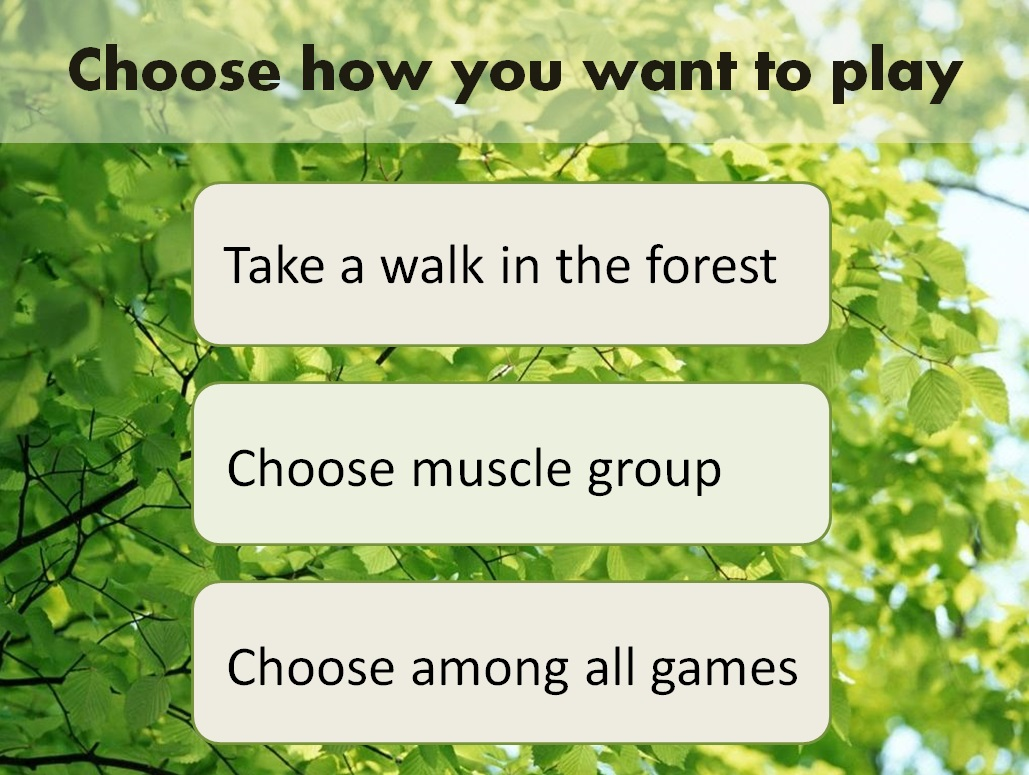
\includegraphics[scale=0.45]{choosePlay.jpg}
\caption[The menu - start]{In the first menu step, the player is given the opportunity to choose how they would like to play. The could go for the compounded game, playing according to a chosen muscle group, or they could choose among the four single games.}
\label{fig:menuStart}
\end{figure} 

\subsection{Exercises}
The activities we have selected for our exergame are based upon findings from workshop 1, and our own ideas, but the main reason for using these activities is because they involve exercises that are shown to be good for elderly. We have used \emph{Øvelsesbanken} \cite{eldretrening}, that we were introduced for in our project \cite{project}, as a guide to find exercises to use in our exergame concept. \emph{Øvelsesbanken} is created by the physiotherapy service in Trondheim, and consists of a set of exercises for elderly that should increase balance and strength. This service is meant to be a tool to help physiotherapists set up customised programs for their older patients. We have picked out 18 exercises from \emph{Øvelsesbanken} that we feel will be a good foundation for our exergame concept. Some exercises chosen are "picking apples", see Figure \ref{pickingapples}, "walking", and "rowing". All the chosen exercises are presented in Appendix B. Most of the exercises have the possibility to be performed both sitting and standing, to make the exergame available for those who are not able to stand or walk.


\begin{figure} [H]
\centering
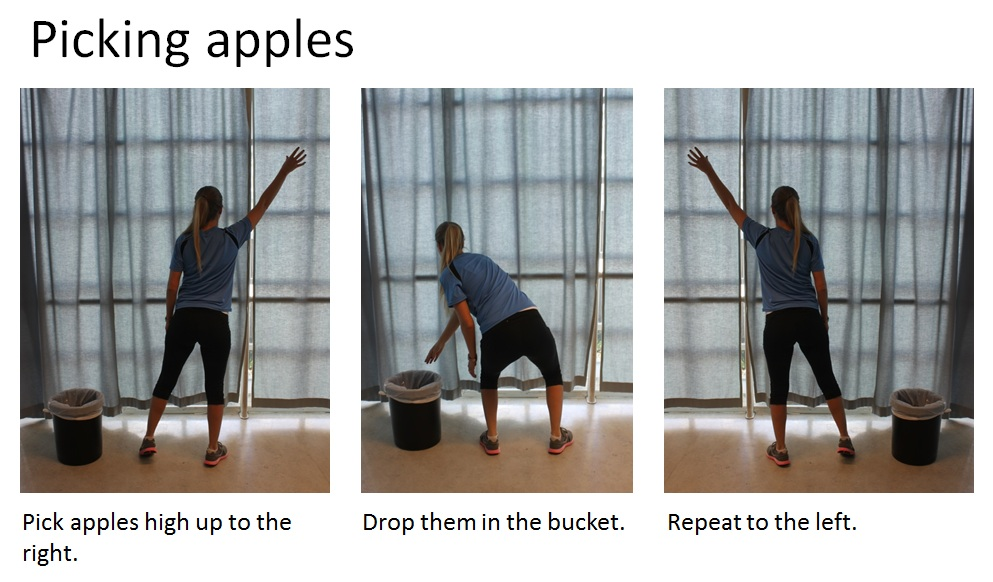
\includegraphics[scale=0.5]{PickingApplesAlone.jpg}
\caption[Exercise - picking apples]{A "Picking apples" exercise from \emph{Øvelsesbanken}.}
\label{pickingapples}
\end{figure}

\subsection{Instruction and Feedback}
In this exergame concept the player will be given sufficient instruction about the technology, how to play, and how to perform various activities and exercises. When first starting the exergame the player will be informed on how to interact with the Kinect sensor and the game. The player will be told that she has to use her body to engage game play, and that she has to use her hand to navigate through the menu. Instruction will be provided on how to interact with the menu, like how to make a choice by "pressing a button". 

In the beginning of each of the five games there will be an instruction informing about the goal of the game, the purpose of the various elements, and how the player should move to perform the activities in the game. All information will not be given all at once, as this will require a lot of memorisation. Therefore, instruction will be given during game play, when there occur situations that makes it appropriate to provide the player with new information. Every instruction will come with a button that the player has to push to continue playing. In this way the player is in the control of the game, and can decide for herself when she is finished reading the instruction. Figure \ref{fig:kineintro} shows an example of an instruction. The player will always be given the possibility to skip the instructions, so the experienced player do not have to watch the same instructions each time she play.

During game play the player will be given appropriate feedback on her actions. This will be given when she have completed a particular task or activity, to not interrupt the player from performing ongoing tasks. An example will be a motivating comment, as "Congratulations, you did a great job", when the player has accomplished balancing over a log. While playing, feedback should be given orally by a calm lady voice. Textual feedback during game play are avoided to not interfere with immersion and disturb the gaming experience.  

\begin{figure} [H]
\centering
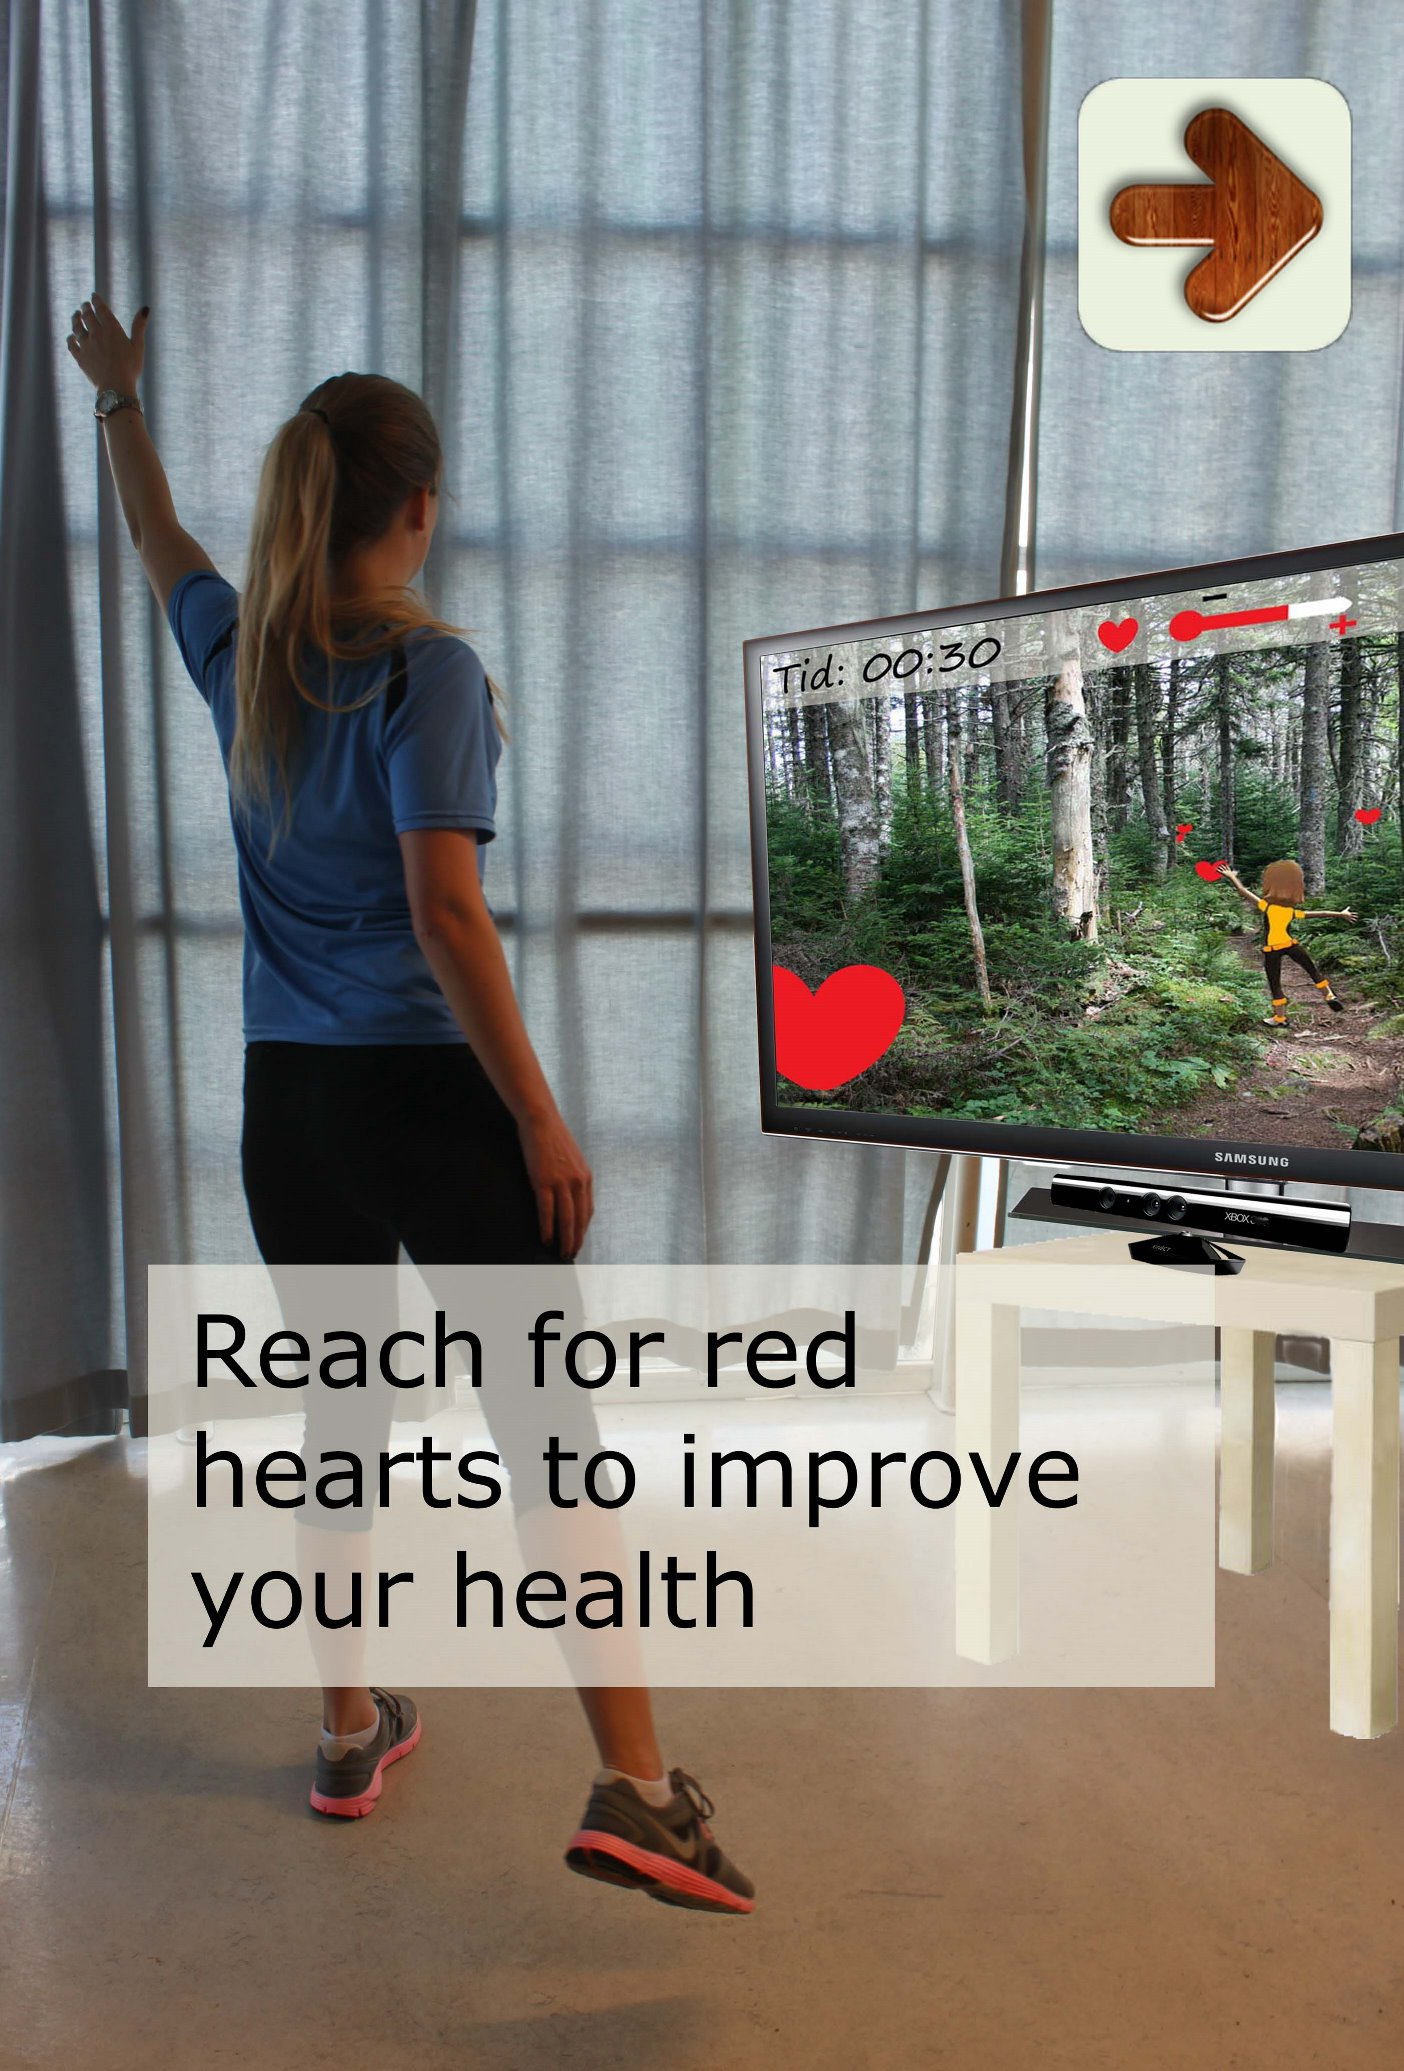
\includegraphics[scale=0.18]{introKineEng.jpg}
\caption[Instruction]{This figure shows an instruction in our exergame concept. There is a button up in the right corner that will be used to continue on with the game when the player is done reading the information.}
\label{fig:kineintro}
\end{figure}

\subsection{Nature Trail}
The main activity in "Out in the Nature", is what we have called a "Nature Trail". This involves a walk in the forest with quizzes along the way. The goal for the game is to complete the nature trail as fast as possible, while answering questions, and avoiding obstacles on the way. Points will be given according to correct answers on the quiz, which will be shown up in the right corner together with a icon showing a sheet of paper. Because the Kinect sensor can track movement, points will also be given according to how well the player performs the required movements. These points will not be shown as numbers, as movements will be difficult to measure and "grade". Therefore, gain from correct and well-performed movements are shown in a "health bar" on top of the screen. A red heart is shown together with the bar to represent health. Points for correct answers on the quiz are separated from points achieved from movements, because the quiz has to do with cognitive skills, while the latter is about physical skills. The time used to complete the nature trail will affect the final result of the "health bar", as this also reflects how well the player has moved during game play. See Figure \ref{fig:hearts} for an example of a scenario, which includes the described elements. The "Nature Trail" supports the possibility to choose number of players, as multi-player mode enhance social interaction while playing.  

Progress in the game requires movement, like walking. When walking, the avatar portraying the player will walk into the forest. The bigger movements the player uses, e.g. the higher the player lift her feet while walking, the higher pace, and "better health" she will achieve. Figure \ref{fig:hearts} shows an avatar in the forest, surrounded by hearts, where the avatar does a wide stretch trying to reach a heart. The hearts will be positioned in a way that will require the player to move to reach for them. Therefore, if the player gathers these hearts, her health will improve due to physical activity. Gain from gathering hearts will also be shown in the "health bar".   

\begin{figure} [H]
\centering
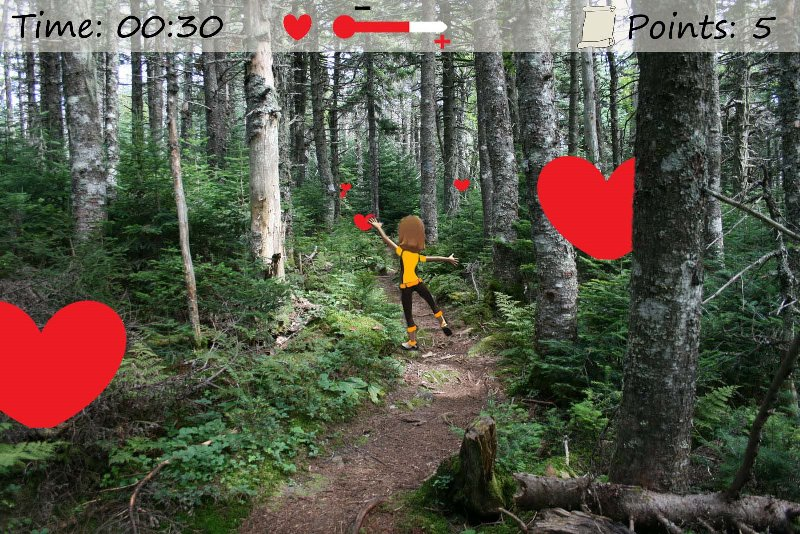
\includegraphics[scale=0.45]{game1engelsk.jpg}
\caption[Nature trail - stretching]{This figure presents a scene from the nature trail. We see an avatar in the forest, doing a wide stretch trying to reach a heart. This will result in improved health, shown in the "health bar".}
\label{fig:hearts}
\end{figure}

The quiz in the nature trail will be shown as sheets of paper "hanging" around on different spots in the forest. The player has to reach for them to get access to the questions, see Figure \ref{fig:quiz}. When picking a question, it will pop up and fill the screen. Four answer alternatives will be shown, and the player will have to user her hand to navigate to what she believes is the right answer. Questions will be chosen randomly, so the player do not get the same questions each time they play. The difficulty will also increase after the amount of correct answers. The player does not have to answer the quiz to complete the nature trail, but it will affect the total score at the end. 

\begin{figure} [H]
\centering
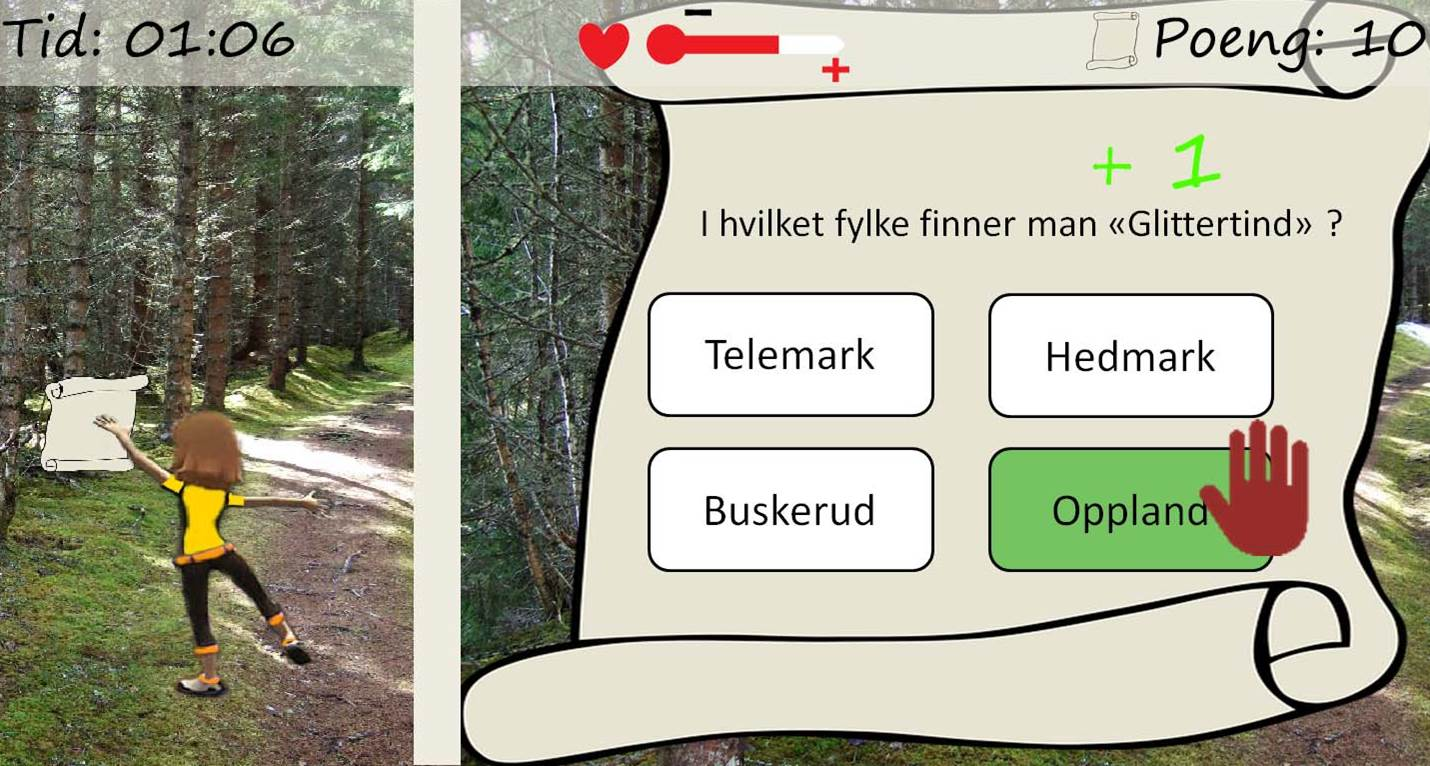
\includegraphics[scale=0.5]{quiz.jpg}
\caption[Nature trail - quiz]{The quiz in the nature trail will be shown as a piece of paper "hanging" on different spots in the game world. Questions will pop up and fill the screen. Here, the player is asked about where to find the Norwegian mountain "Glittertind".}
\label{fig:quiz}
\end{figure} 

Along the way in the nature trail there will be various, natural obstacles that will force the player to move her body in certain ways to be avoided. The obstacles have been chosen according to which movements that are required by the player, as the nature trail is supposed to train the whole body. Examples of these obstacles are a river or creek that the player has to cross, or logs or rocks lying on the path that the player has to step over. To cross a river or creek the player has to balance on logs or step on rocks. This requires movements as toe-to-heel stepping, and step touch or skaters. When meeting a log, the player is required to take a big step, or a lunge, to get past it. Rocks in the path is avoided by performing sideways steps, or step touch. There will also be obstacles in head hight, like branches, which requires the player to go into deep squats to avoid them. The Kinect sensor will track the player's body, and increase or decrease the "health bar" according to how well the player perform the required movements. If the player hits some of the obstacles, they will get a flash of red, indication that the player failed to avoid them. As a result, the "health bar" will decrease.

The story is organised with the use of "branching", which is about having the possibility to choose between multiple paths. An example of this is choosing between walking the "regular" trail or rowing a boat over a lake. When meeting the lake, there will be a rowing boat by a pier on the water. To cross the lake, and continue the nature trail, the player has to take a side step and step into the boat. To move forward, rowing movements are needed. There will be water lilies in the water which the player has to avoid. This is done by leaning the upper body over to the sides. This, and all the other described obstacles, are shown in Figure \ref{fig:hindringerEng}. All the tasks the player has to do throughout the game will be described in the functional design, in Section \ref{sec:designnature}. The reader is referred to Appendix B for detailed instructions on how to perform the various exercises.

\begin{figure} [H]
\centering
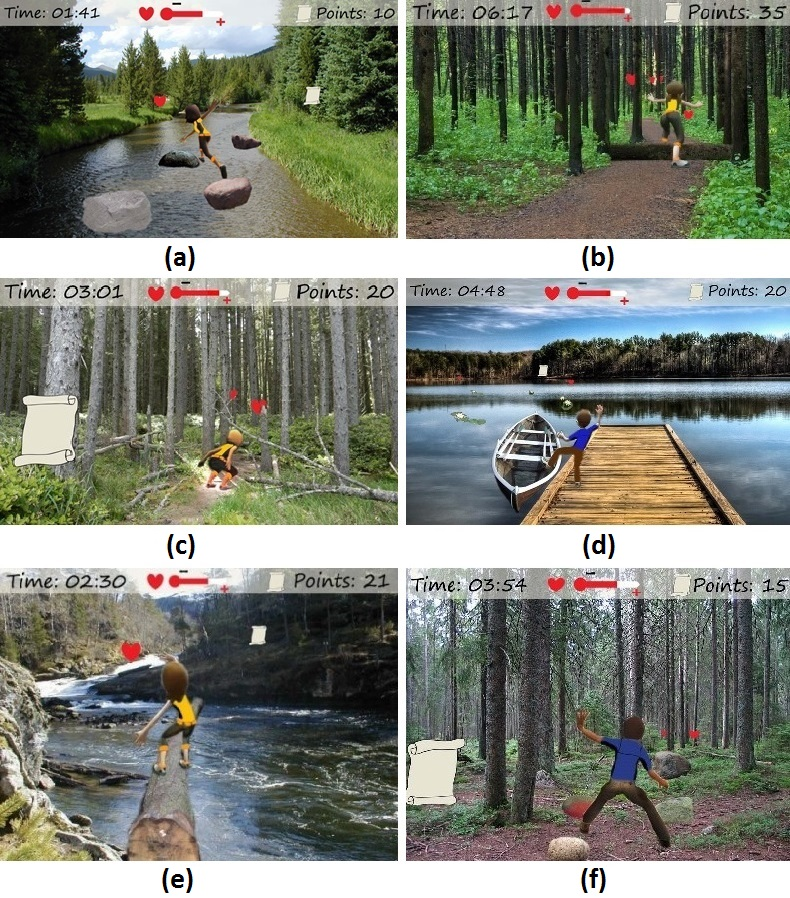
\includegraphics[scale=0.6]{hindringerEng.jpg}
\caption[Nature trail - obstacles]{This figure presents various obstacles to be found in the nature trail.}
\label{fig:hindring}
\end{figure}

One of the requirements for this exergame concept is that the game has to show progress. In workshop 1, the informants told us that it was important to see that they learned something, and that they got better. They also expressed it as important to get the possibility to choose difficult levels themselves. We have solved this by having a step in the menu where the player can choose the preferred difficulty for the game, see Figure \ref{fig:omgivelseNivaa}. 

\begin{figure} [H]
\centering
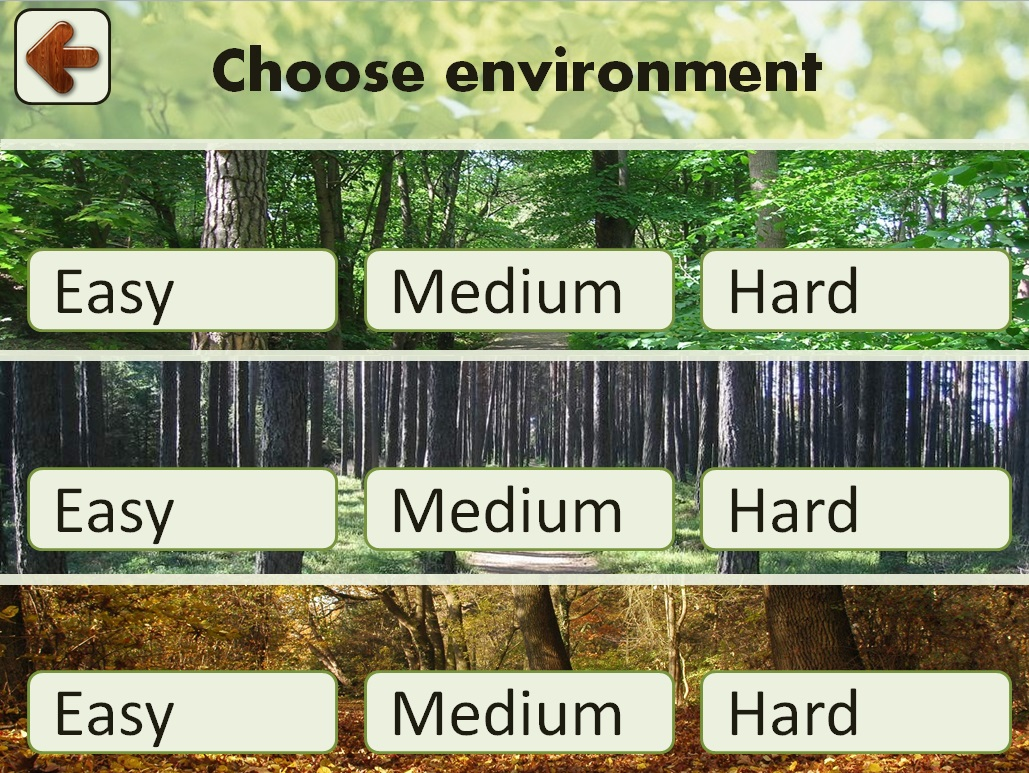
\includegraphics[scale=0.45]{chooseEnvironment.jpg}
\caption[Choice of environment and difficulty level]{When "Take a walk in the forest" is chosen, players will get the possibility to choose environment and difficulty level. The environments to choose from are pine wood, deciduous wood summer, and deciduous wood fall. Within each environment there are three difficulty levels.}
\label{fig:omgivelseNivaa}
\end{figure}

The nature trail offers three different forest environments to walk in, a pine wood, and two deciduous woods, showing both summer and fall. Each of the environments presents initial, different difficulty levels, and within each environment, there are three difficulty levels, easy, medium, and hard. First time playing, only the easy level will be available. The higher levels will be unlocked when the player has managed the easier level. A higher difficulty level will require more from the player, both mentally and physically. Obstacles will occur more frequently, which will require concentration, and the movements and exercises will be harder to perform, and therefore require control of the body. Within one environment the obstacles from the easy level will follow to the next levels. This is done to include some familiar elements in the higher levels, in addition to the new obstacles that will be added. To at the same time support variation between the environments, new and different obstacles will be used in each of the three environments.  

Required movement during the nature trail we now have presented will exercise the whole body. This involves endurance, balance, and exercise of several muscle groups. This nature trail, with the quiz and movements combined, will be good for both cognitive skills and improved physical health.     


\subsection{The Four Single Games}
In addition to the nature trail, "Out in the Nature" consists of four shorter games with focus on completing one single activity or challenge. The activities we have chosen for our exergame concept are wood chopping, paddling down a river, swimming in a lake, and picking apples. Within every game the player has the possibility to choose number of players and difficulty level. In multi-player mode, players can choose if they want to cooperate or compete against each other. When competing, the players will have the possibility to select difficulty level individually. This is to allow for players with different experience to play together, like an elderly and her grandchild. Figure \ref{fig:velgSpill} shows how these single games will be presented in a menu. We will describe one of these four games in more detail.

\begin{figure} [H]
\centering
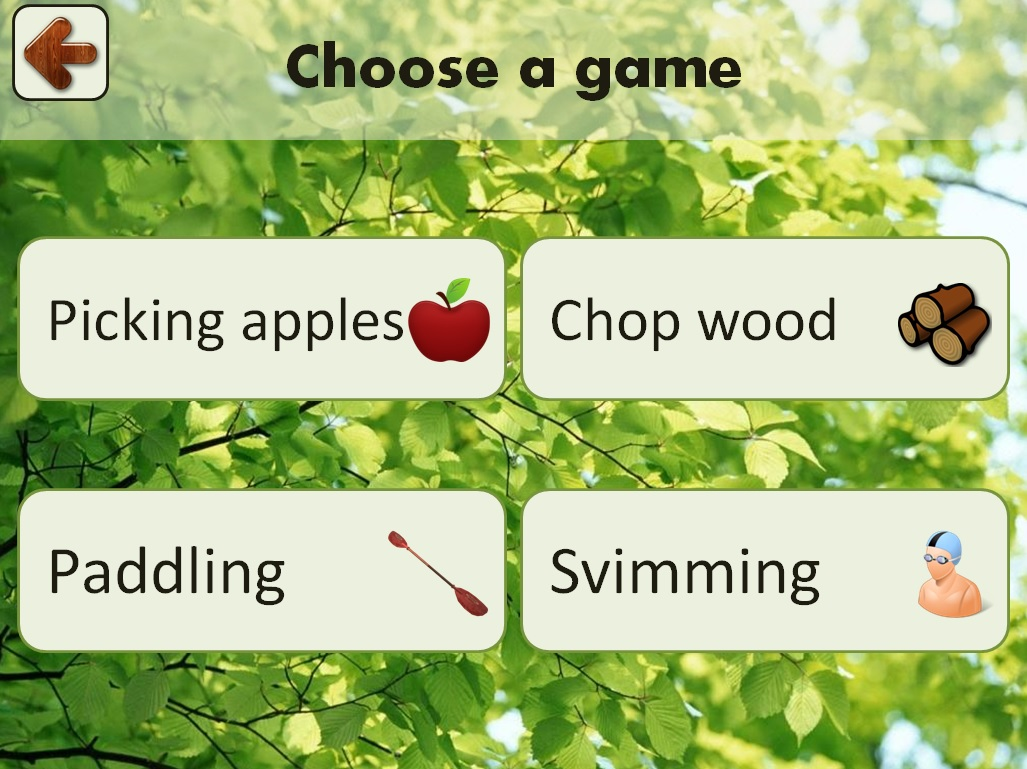
\includegraphics[scale=0.4]{chooseGame.jpg}
\caption[The four single games]{Besides the walk in the nature the players can choose between four single games, picking apples, chopping wood, paddling, and swimming.}
\label{fig:velgSpill}
\end{figure}

\subsubsection{Picking Apples}
"Picking Apples" is a game that requires squats and stretching exercises, which will strengthen balance and muscles in thighs and the gluteal area. The goal for this game is to pick as many red, ripe apples as possible in a given amount of time, and the apples should be put in baskets on the ground. This is shown in Figure \ref{fig:appleStretch} and \ref{fig:appleSquat}. The movements this game requires fits well with the exercise chosen from \emph{Øvelsesbanken}, see Figure \ref{pickingapples}. When apples first appears on the tree they will be green, indicating that they are not ready to be picked. If ripe apples are left hanging on the tree for too long, they will rot and fall to the ground. Rotten apples will have a brown color. 

\begin{figure} [H]
\centering
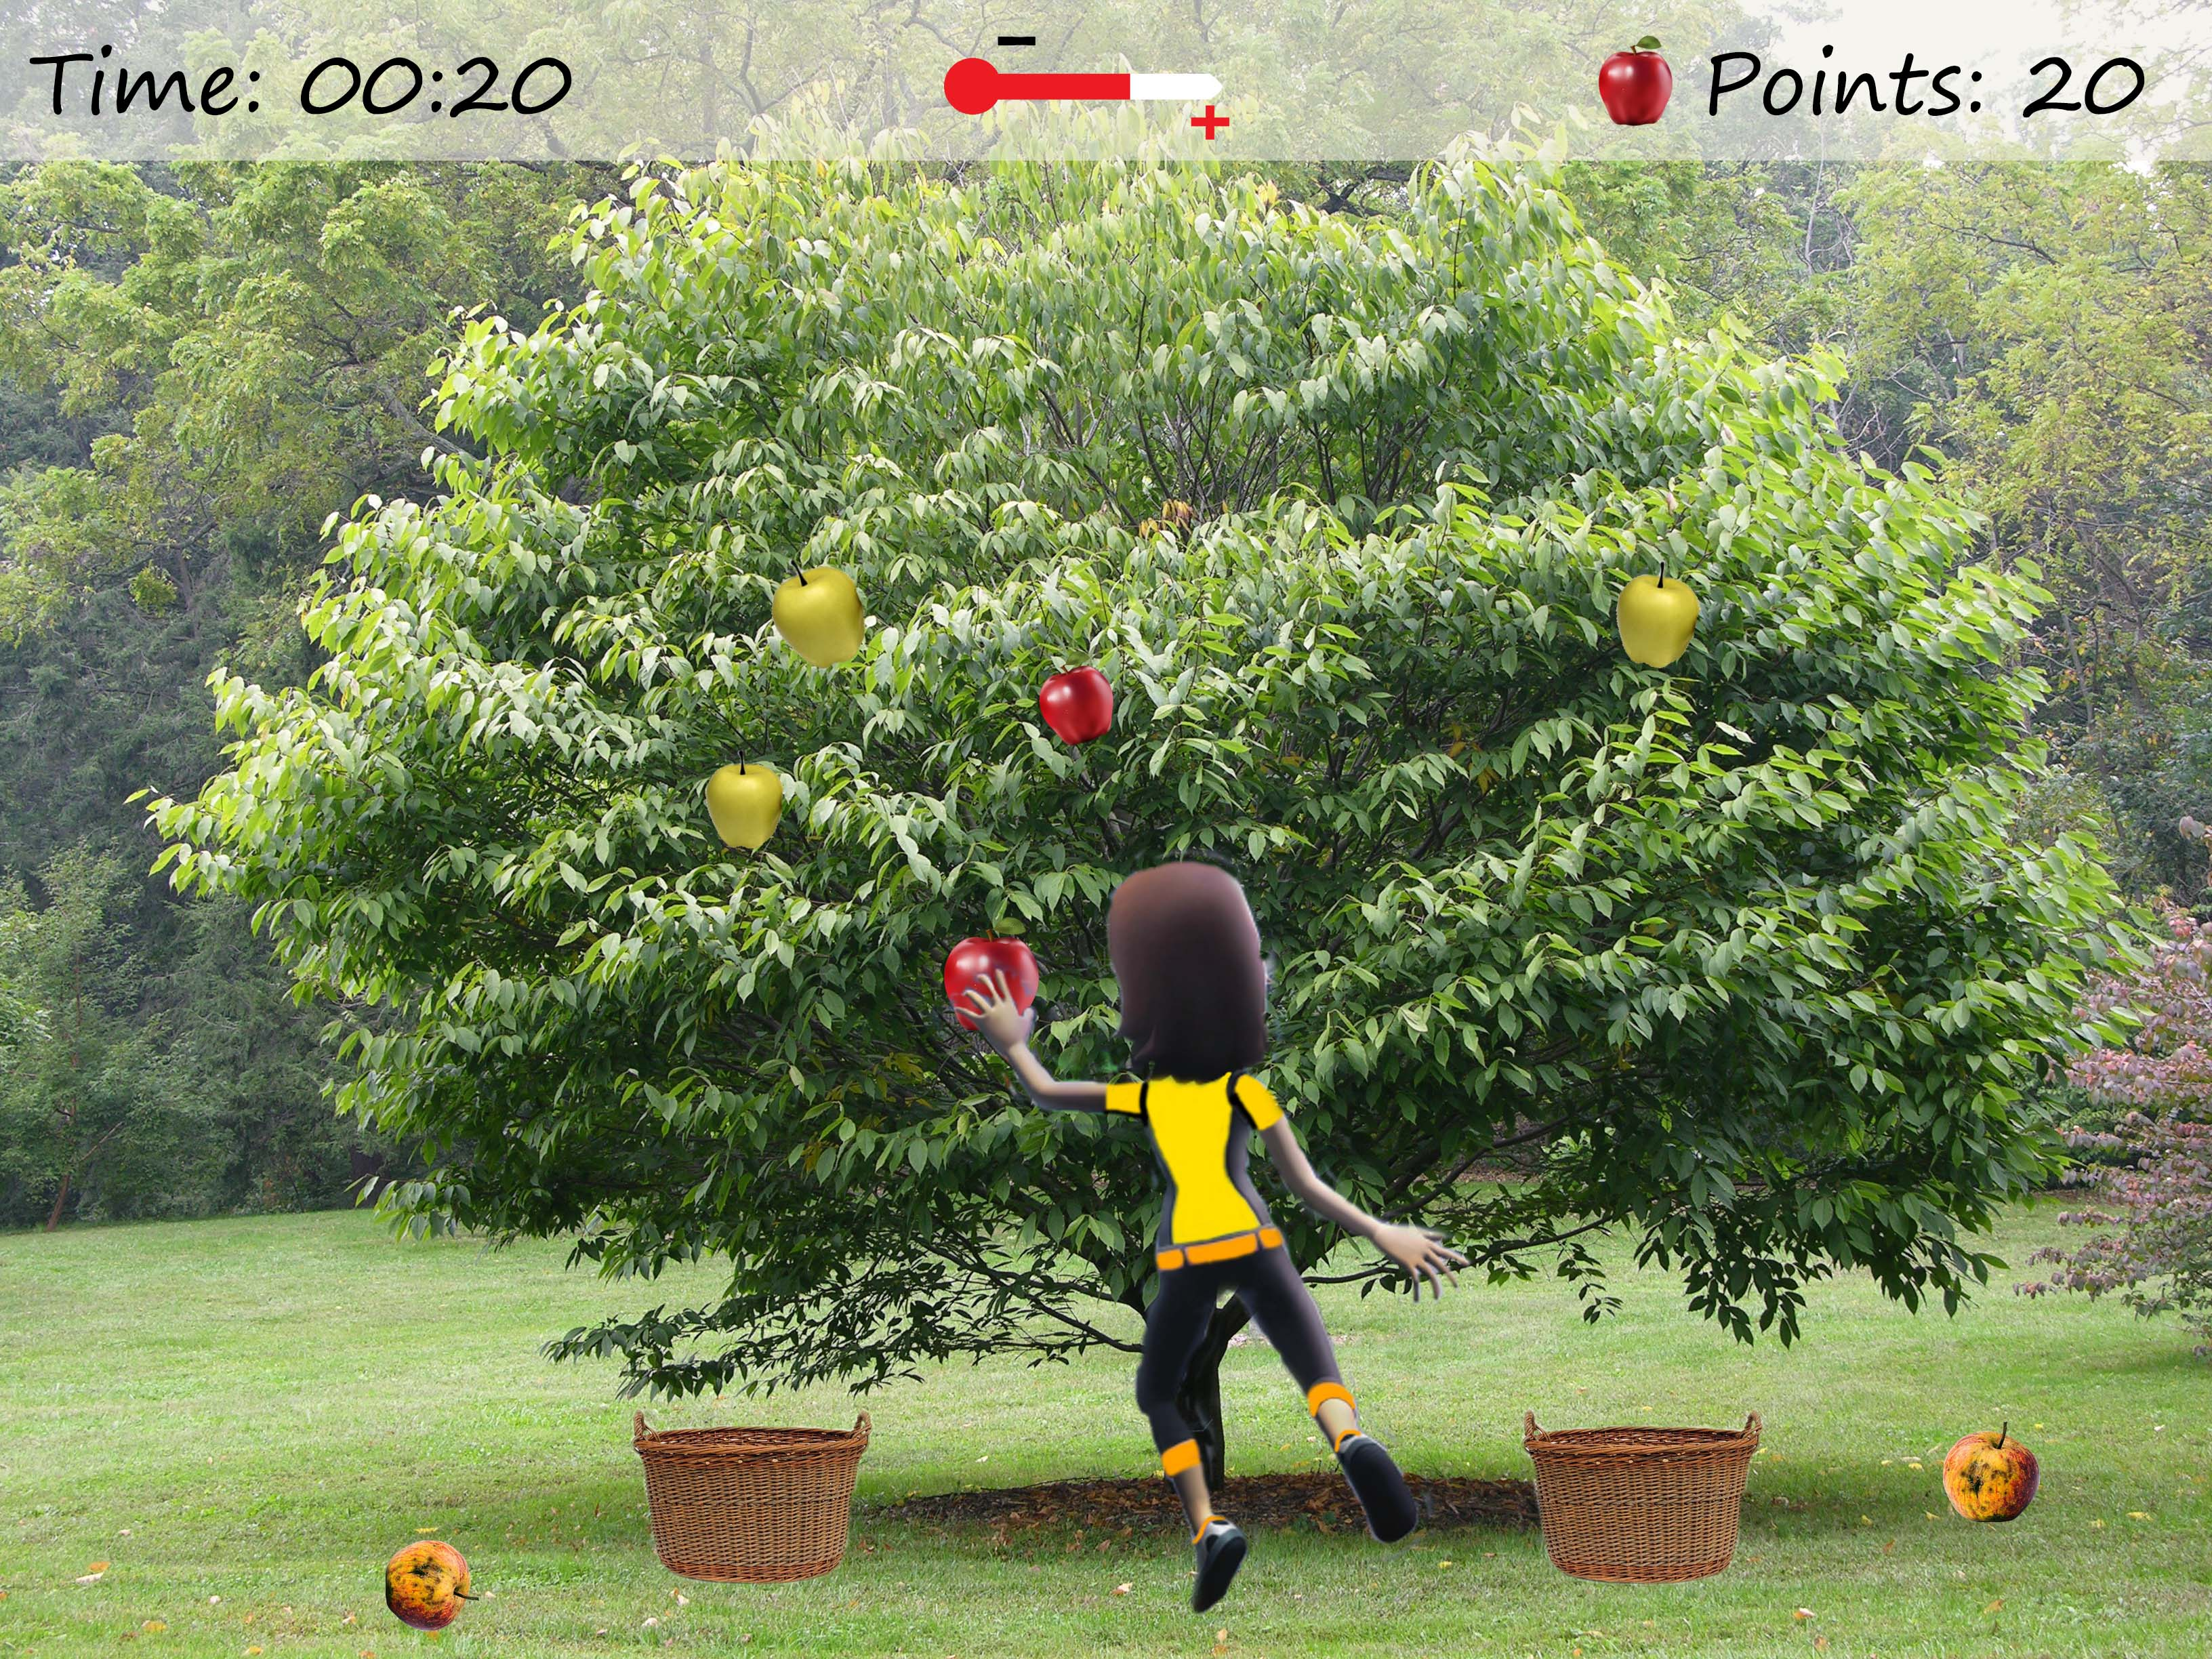
\includegraphics[scale=0.1]{gameappletreeEng.jpg}
\caption[Picking apples - stretching]{The player stretch up to pick a red, ripe apple. We observe that there are, in addition to red apples, three green apples on the tree, and two rotten on the ground.}
\label{fig:appleStretch}
\end{figure}

\begin{figure} [H]
\centering
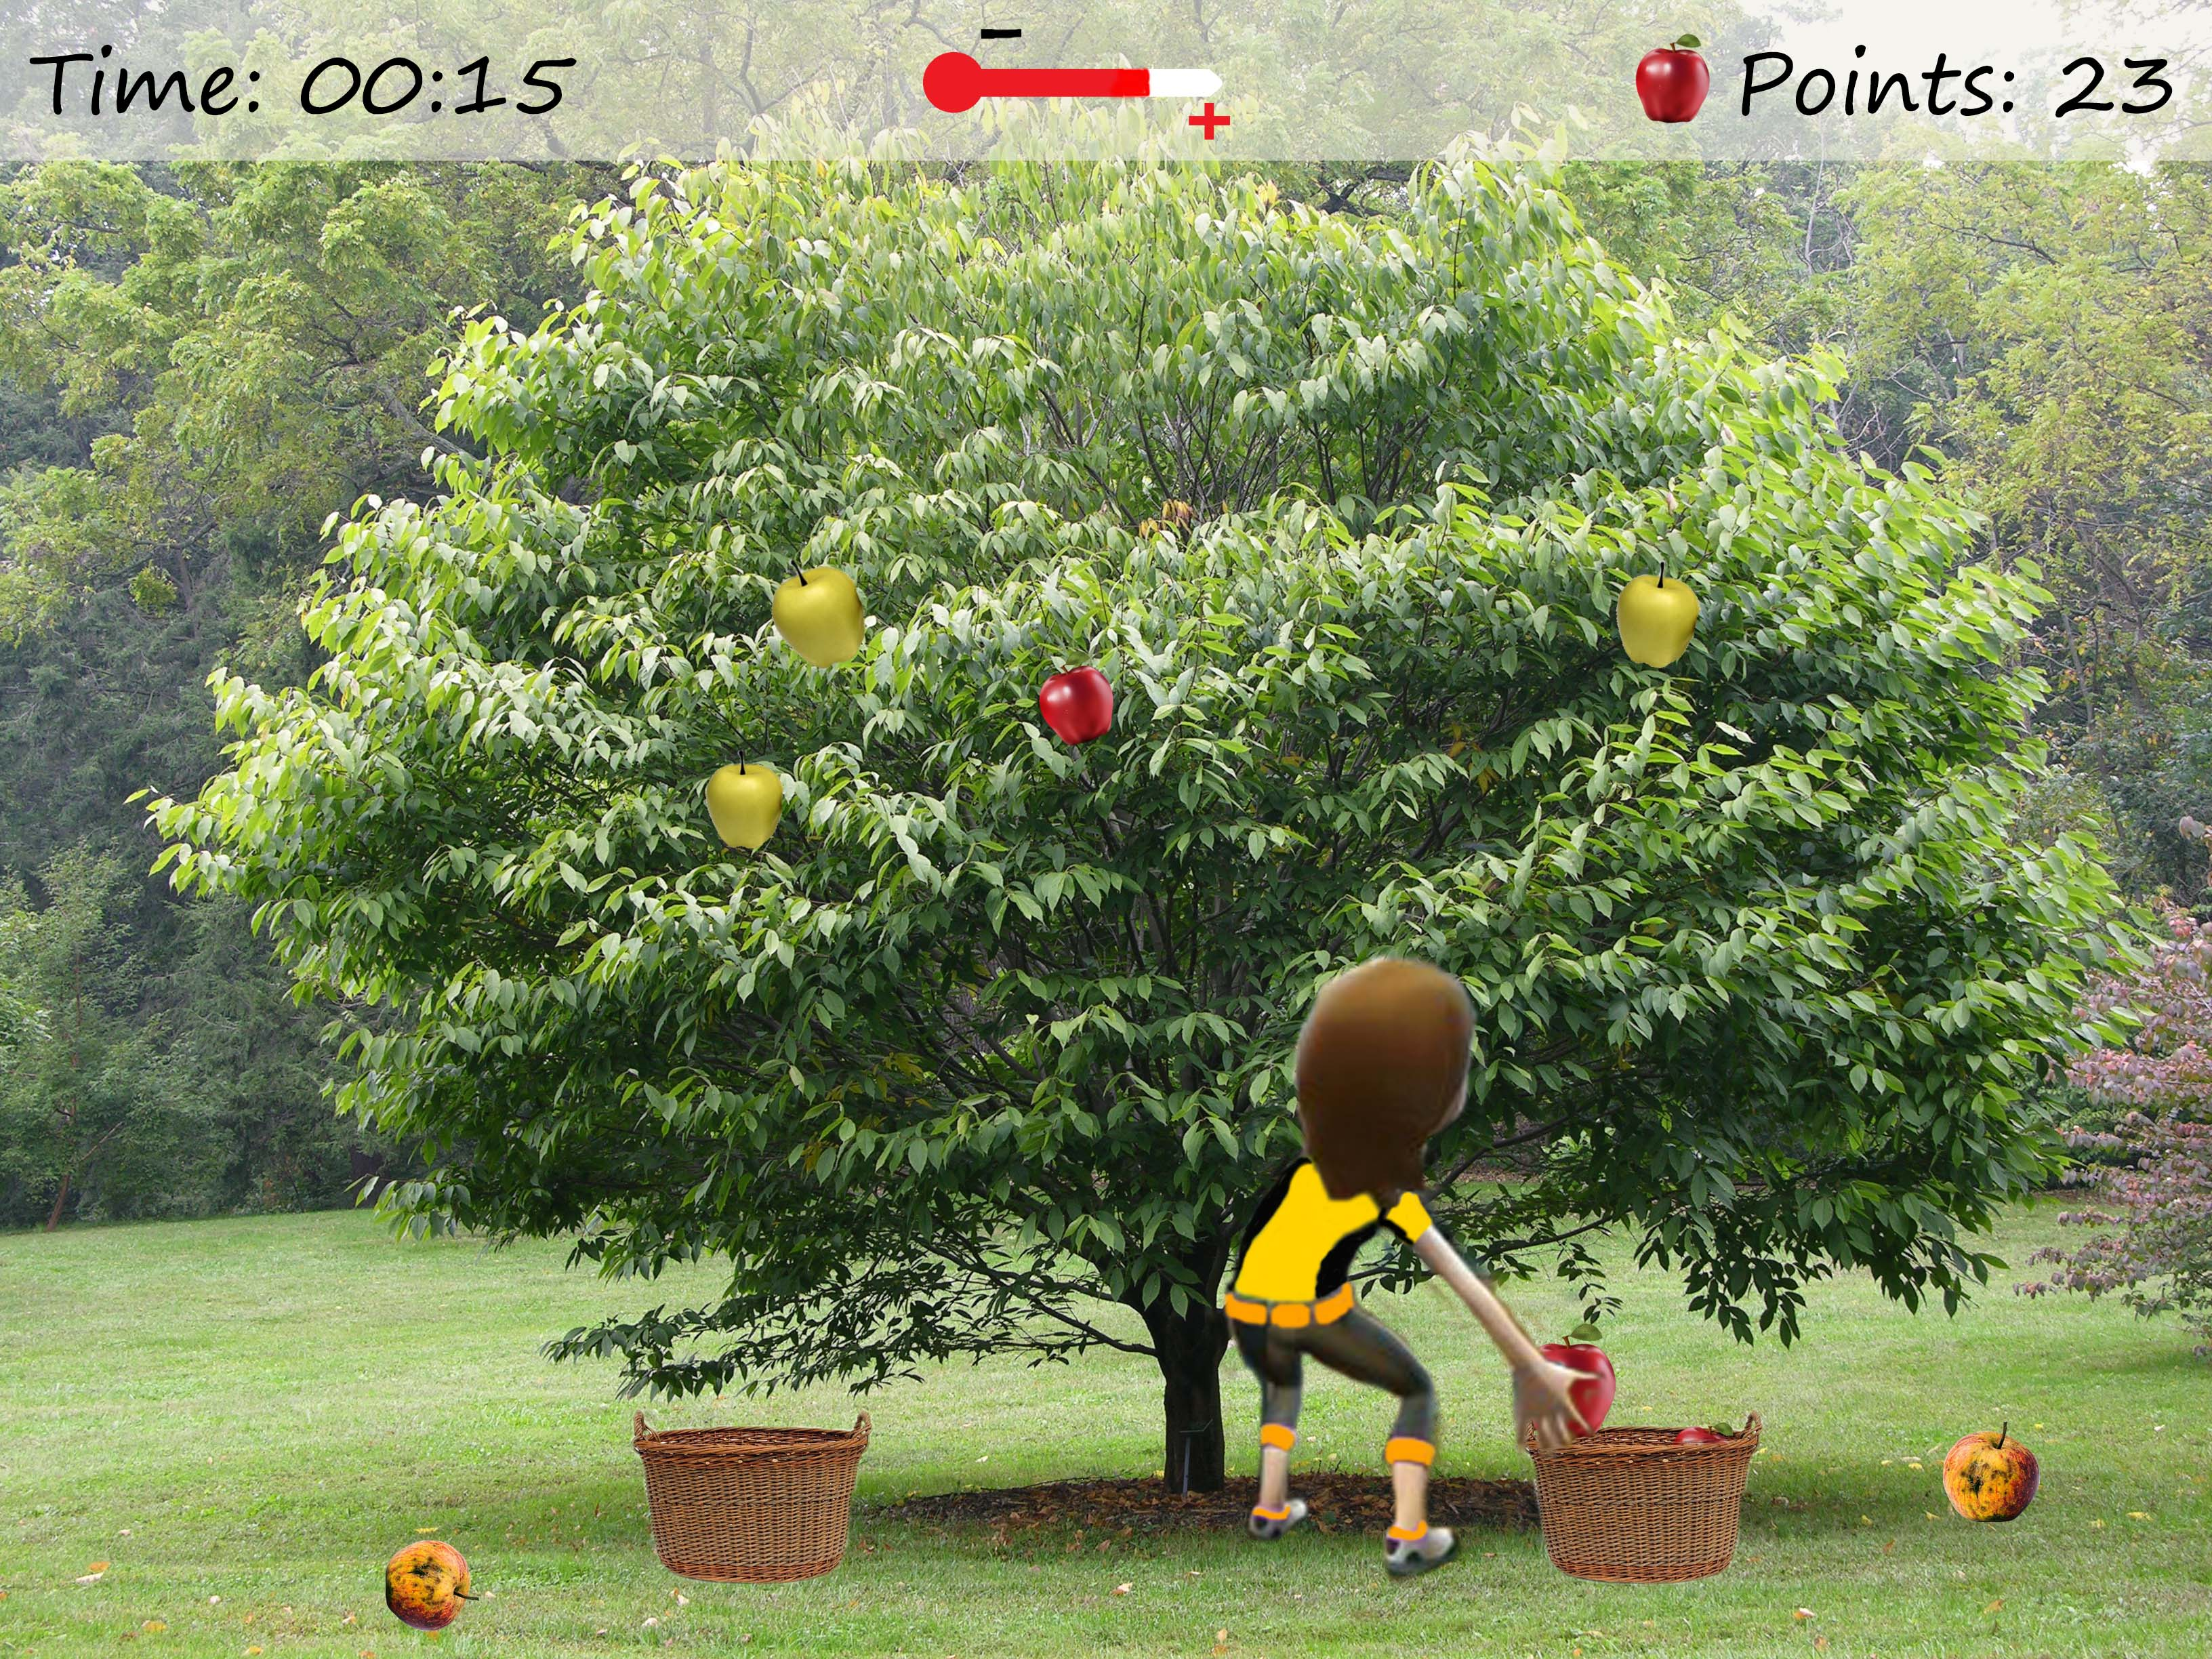
\includegraphics[scale=0.1]{squatppletreeEng.jpg}
\caption[Picking apples - squats]{The player has picked a red apple and is about to put it in the bucket. The player use deep squats.}
\label{fig:appleSquat}
\end{figure}

Points will be given according to how many apples the player has picked, see Figure \ref{fig:appleOver}. 3 points will be given for each ripe apple that is picked and put in a basket. The player will loose points if green apples are picked, or if apples have been given the time to rot. Picking a green apple will result in -1 point, and if the apple gets rotten this will result in -2 points. If the player does not perform squats when putting apples in a bucket, there is a great possibility that the apple will miss the bucket and fall to the ground. This will give the same loss of points as a rotten apple, -2 points.       

\begin{figure} [H]
\centering
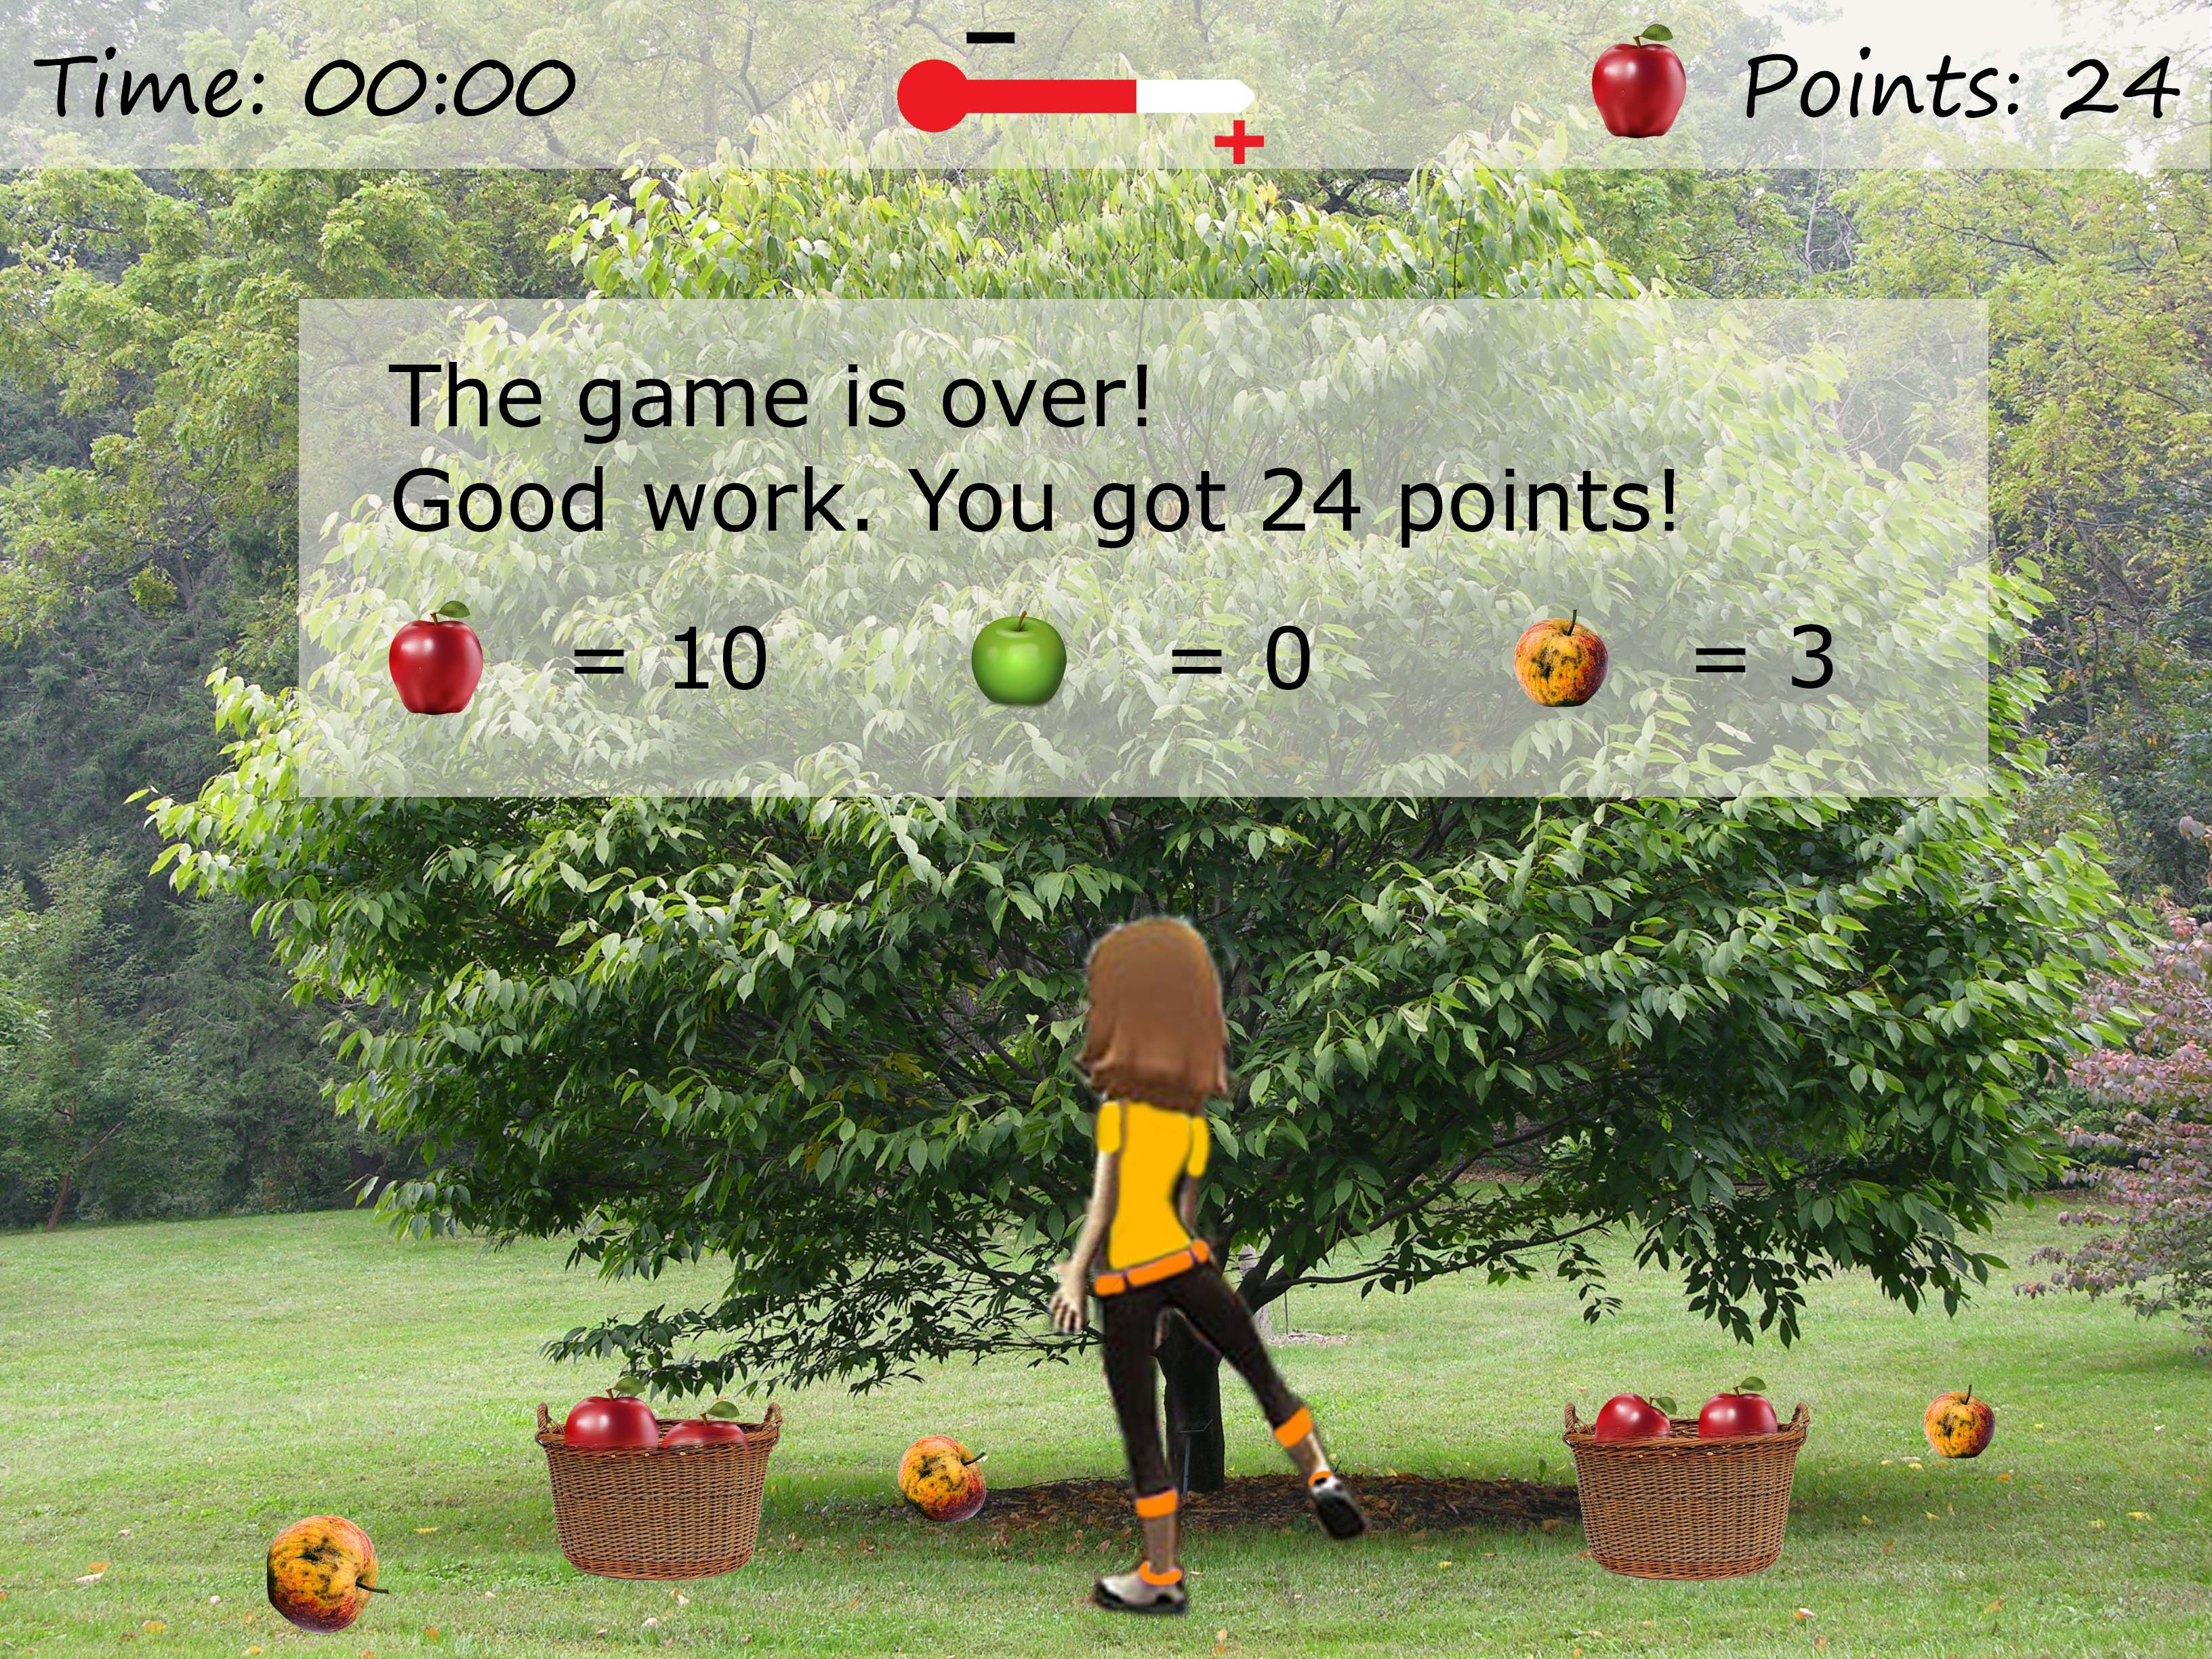
\includegraphics[scale=0.1]{appletreeendEng.jpg}
\caption[Picking apples - points]{This figure presents a final scene in the "Picking Apples" game. A text together with the number of apples picked, are shown.}
\label{fig:appleOver}
\end{figure}

Apples will appear on the tree and grow in a certain tempo according to the chosen difficult level. Higher difficulty will result in more apples on the tree at the same time, and a faster ripening rate. An extra challenge to be added at a higher difficulty level is requirements to which of the two buckets the newly picked apple should be put. This is to train cognitive skills and to include more variation in movements and exercises. As mentioned, this game allows for multi-player mode where the players could collaborate on picking apples, or compete on who can pick the most apples, see Figure \ref{fig:appleMultiplayer}. 

\begin{figure} [H]
\centering
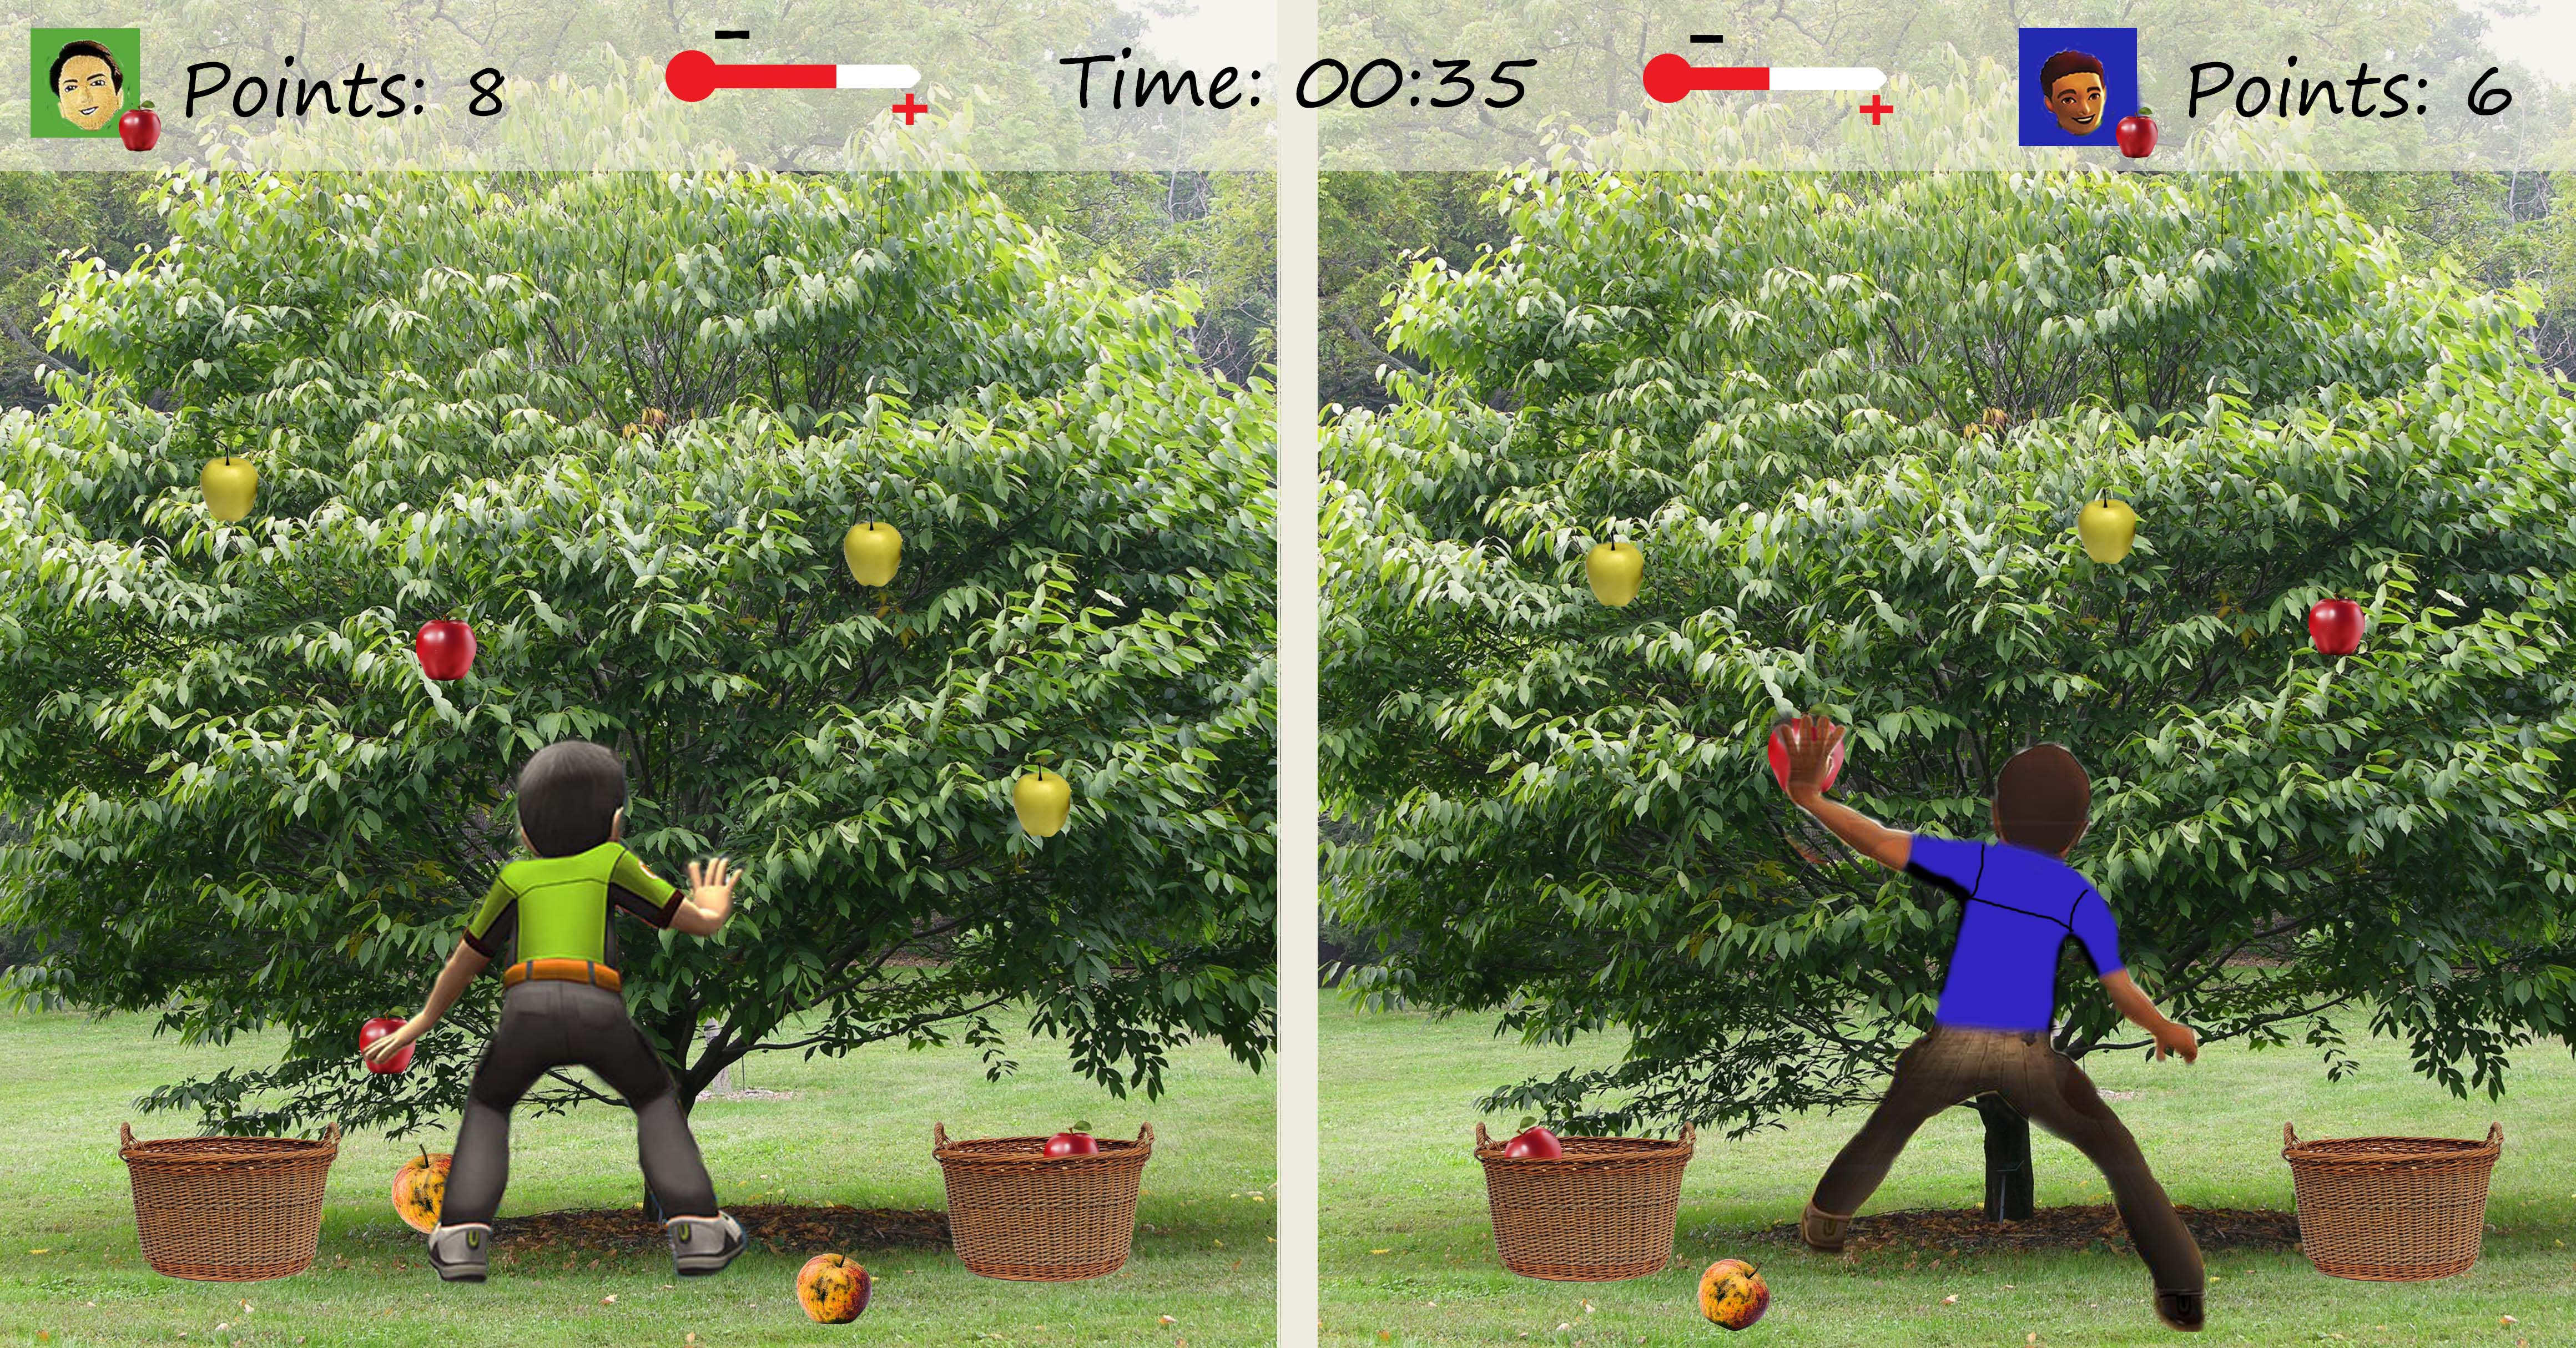
\includegraphics[scale=0.075]{gameapple2playerEngelsk.jpg}
\caption[Picking apples - multi-player]{In this figure we observe two players playing together in competitive mode.}
\label{fig:appleMultiplayer}
\end{figure}

\section{Functional Design}
\label{sec:functionaldesign}

The functional design for this game will be described according to system requirements presented in Section \ref{sec:req}, and to video game theory discussed in Chapter \ref{chap:vg}. The functional design will provide a more concrete representation of the exergame concept than what have been presented earlier in this chapter. Here, all the elements the game should contain will be presented shortly. Functional design will vary according to the chosen difficulty level, however, in this thesis we will only focus on presenting functional design for one difficulty level.

We will describe functional design for what we have presented in the exergame concept, hence, the "Nature Trail" and "Picking Apples". This will, as mentioned, be described according to Chapter \ref{chap:vg}, more specific, according to the game's story and aesthetics.  

\subsection{Nature Trail}

\subsubsection{The Fictional World} 

\begin{table} [H]
\centering
    \begin{tabular}{|p{3,2cm}|p{7,8cm}|}
       \hline
        \emph{Location/setting} & In the forest  \\ \hline
       \emph{Structural objects} & Trees, the trail, heaven, rocks, log, anthill, lake, puddle, creek, river.  \\ \hline
       \emph{Interactive objects} & The player character, row boat with oars, rocks lying in the middle of the trail, rocks in the river, logs over a creek, red hearts in the field, bought, question sheets. \\ \hline
	   \emph{Scripting objects} & Quiz points: Shown as an icon similar to a sheet of paper, with the text "points" after it. Increments with 5 points as the player answer the right question.\\ \hline
	     & "Health-bar": Increase as player performs right movements. Decrease as player do not manage the right movements. Increase when player gather hearts. Increase based on time spend in game world compared to previous sessions. 
	      \\ \hline
	       & Time: Increases as a normal clock \\ \hline
	       \emph{Characters} & An avatar (from how Kinect defines a character) seen in third-person perspective, described by its name. \\ \hline
    \end{tabular}
    \caption[Various objects in the "Nature Trail"]{Different types of objects}
    \label{tab:objects1}
\end{table}  

\subsubsection{Mechanics} 

The game is a progression game, where a story should be solved. Each level will be completed by solving puzzles. The player has to finish different quests within a level to proceed to the next level, and the levels are building on each other. It is common to have a climax at the end of each chapter in these type of games. However, this is not included here, as this will interfere with the natural environment and the gaming experience for this type of users. In Table \ref{tab:quests1} we will present different quests in this game. 
  
\begin{table}
     \begin{tabular}{|>{\raggedright}p{3,5cm}|>{\raggedright}p{4cm}|p{3,5cm}|}
       \hline
        \textbf{What do do} & \textbf{Goal} & \textbf{Exercise required}  \\ \hline
       Walk the trail & Get forward in the game world & Lift legs high, walking  \\ \hline
       Gather hearts & Use body to get heart and "get better health" &  Stretching \\ \hline
	   Watch out for rocks lying in the middle of the trail & Change movements to get forward & Side steps or step touch  \\ \hline
	     Watch out for branches hanging over the trail & Change movements to get forward & Squats
	      \\ \hline
	       Balance over a log that lies over a creek & Change movements to get to the other side of the creek & Toe-to-heel stepping with arms out \\ \hline
	       Get over the log lying across the trail & Change movements to get forward & Lunges \\ \hline
	       Jump from rock to rock to get over the creek & Change movements to get to the other side of the creek & Step touch or skaters \\ \hline
	       Row boat over to the other side of the lake & Change movements to get over the lake  & Rowing \\ \hline
	       When rowing watch out for the water lilies & Change movements to get over the lake without hitting the lilies  & Lean upper body from side to side \\ \hline
	       Find question sheets & Use body to get question sheet  & Stretching \\ \hline
	       Answer one of the four answer alternatives & Answer the right question  & Use knowledge and cognitive skills \\ \hline
	       Solve puzzle & Solve puzzle right  & Use knowledge and cognitive skills \\ \hline
      \end{tabular}
      \caption[Quests in the "Nature trail" game]{Quests}
    \label{tab:quests1}
 \end{table}
 
\emph{Branching} \\ \\ 
"Branching": Trail splits, and there are two possibilities: 1. Walk one trail with rock obstacles but a lots of hearts to gather. This will require some more time, but the player can gain more points by gathering hearts. 2. Walk the other trail which is without obstacles but no hearts to gather. 

"Branching": Trail splits, and there are two possibilities: 1. Keep walking the trail. 2. Row a boat over to the other side. Rowing requires legs wide apart and arms stretched out in front of the player and dragged back to their body, as actual rowing movements. 

\subsubsection{Rules} 
 
\begin{table} [H]
\centering
    \begin{tabular}{|p{2,8cm}|p{8,2cm}|}
       \hline
	   \emph{Interplay rules} & \textbf{1. The player character:} will move to the movements received as player input. \\ \cline{2-2}
	     & \textbf{2. Rowboat with oars:} will move forward as the player  uses her arms with the oars. \\ \cline{2-2}
	       & \textbf{3. Rocks lying in the middle of the trail:} If hit, the  rocks will flash red.  \\ \cline{2-2}
	        & \textbf{4. Log over creek:} If the avatar falls off, the log will flash red. The player will automatically get up on the log again. \\ \cline{2-2}
	        & \textbf{5. Rocks in river:} If the avatar miss a rock and fall of, the rock will flash red. The player will automatically get up on the side of the river again. \\ \cline{2-2}
	         &  \textbf{6. Red hearts:} When touched by the avatar it disappears. \\ \cline{2-2}
	          &  \textbf{7. Bought:} If hit, it will flash red \\ \cline{2-2}
	           &  \textbf{8. Question sheets:} When touched by the avatar  it  disappears from the game world and fills the screen with  a  question or puzzle. \\ \hline
	            \emph{Evaluation rules} & \textbf{if 1}: Player gets forward in the game, and health-bar fills with red color. \\ \cline{2-2}
	               & \textbf{if 2:} Player gets forward in the game, and the health-bar fills with red color.   \\ \cline{2-2}
	               & \textbf{if 3:} Player gets slowed down, and red color in the health-bar reduces.   \\ \cline{2-2}
	               & \textbf{if 4:} Player gets slowed down, and red color in the health-bar reduces   \\ \cline{2-2}
             	   & \textbf{if 5:} Player gets slowed down, and red color in the health-bar reduces.   \\ \cline{2-2}
	               & \textbf{if 6:} Health-bar fills with red color.  \\ \cline{2-2}
	               & \textbf{if 7:} Player gets slowed down, and red color in the health-bar reduces.  \\ \cline{2-2}
	               & \textbf{if 8:} If player answers right she gets +5 points. If player answers wrong she gets 0 points.  \\ \hline
    \end{tabular}
    \caption[Rules in the "Nature Trail" game]{Rules}
    \label{tab:rules1}
\end{table}  

\subsubsection{Geography and Representation}

\begin{table} [H]
\centering
    \begin{tabular}{|p{2,7cm}|p{8,3cm}|}
       \hline
       \emph{Music} & Calm, classical music that changes to the speed of the game and to certain happenings. \\ \hline
       \emph{Vocalization} & The avatar will not have its own voice. \\ \hline
       \emph{Sound effects} &  When hearts are gathered there is a cheerful "pling" sound.  \\ \cline{2-2}
	    &  When taking the question sheet there is a "swosj" sound.\\ \cline{2-2}
	     & When the character is walking there is the sound of steps on the ground. Different sounds for \\ & different surface, like walking on the rocks, earth or logs.\\ \cline{2-2}
	       & The sound of shoved water when rowing. \\ \hline
	       \emph{Ambient effects} & Birdsong. \\ \cline{2-2}
	         & Wind. \\ \cline{2-2}
	         & Water flowing in the river. \\ \cline{2-2}
	         & Waves from the lake.\\ \hline
	         \emph{Feedback} & Calm lady voice. \\ \hline
    \end{tabular}
    \caption[Different types of sound]{Different types of sound}
    \label{tab:sound1}
\end{table}  

\begin{table} [H]
\centering
    \begin{tabular}{|p{2,5cm}|p{8,5cm}|}
       \hline
      \emph {Perspective} & Third-person. \\ \hline
       \emph{Dimension} &  3-dimensional and isometric. \\ \hline
	       \emph{Exploration} & Desired pace. \\ \hline
	       \emph{Time} & The game time will behave as a normal clock, counting upwards. \\ \hline
	       \emph{Graphical representation} & The environment will be presented as close to photorealism as possible.  However, there will be some unrealistic elements present in the game world.  \\ \hline
    \end{tabular}
    \caption[Graphical game characteristics]{Graphical game characteristics}
    \label{tab:graphical1}
\end{table}  

\subsubsection{Number of Players}
The game supports two simultaneous players. The players can either compete or cooperate.

\subsection{Picking Apples}

\subsubsection{The Fictional World} 

\begin{table} [H]
\centering
    \begin{tabular}{|p{3,2cm}|p{7,8cm}|}
       \hline
        \emph{Location/setting} & Standing on a lawn with a apple tree in front of the player. \\ \hline
       \emph{Structural objects} & Tree, grass, heaven.  \\ \hline
       \emph{Interactive objects} & Apples on the tree, two baskets, one on each side of the player. \\ \hline
	   \emph{Scripting objects} &  Points: Shown as an apple icon with the text "points" after it. Increments with 3 points as ripe apples are picked and decrements with -1 point if a unripe apple is picked, and -2 points if an apple gets rotten \\ \cline{2-2}
	   & "Health-bar": Increase as player performs right  movements. Decrease as player do not manage the right  movements.  \\ \cline{2-2}
	   & Time: Decrease from 2 minutes \\ \hline
	   \emph{Characters} & An avatar (from how Kinect defines a character) seen in third-person perspective, described by its name. \\ \hline
    \end{tabular}
    \caption[Various objects in the "Picking Apples" game]{Different type of objects}
    \label{tab:objects2}
\end{table}  
 
\subsubsection{Mechanics} 
This is a progression game where different levels of the game is finished by solving the apple-picking task. Player has to finish different levels to proceed to the next level. The levels are building on each other and the difficulty level get higher as the player proceeds through the game.

\emph{Quests:} 

\begin{table}
     \begin{tabular}{|>{\raggedright}p{3,5cm}|>{\raggedright}p{4cm}|p{3,5cm}|}
       \hline
        \textbf{What do do} & \textbf{Goal} & \textbf{Exercise required}  \\ \hline
       Pick apples when they get red and ripe. & Pick as many ripe apples as possible and move body & Stretching  \\ \hline
       Put ripe apples in baskets & Fill baskets with ripe apples and move body &  Squats with downward arm movement \\ \hline
      \end{tabular}
      \caption[Quests in the "Apple Picking" game]{Quests}
    \label{tab:quests2}
 \end{table}

\subsubsection{Rules} 

\begin{table} [H]
\centering
    \begin{tabular}{|p{2,8cm}|p{8,2cm}|}
       \hline
        \emph{Interplay rules} &  \textbf{1. apples on the tree:} Will appear on the tree with a yellow-green color showing they are not yet ripe. After a while they will start to get red, and if the apples does not get picked while they are red, they will become brown and fall to the grown. \\ \cline{2-2}
	     & \textbf{2. baskets:} The baskets will get filled with apples. \\ \hline
	     \emph{Evaluation rules} & \textbf{if 1:} If player picks a ripe apple she gets +3 points. If apple becomes rotten player gets  -2 points. If player picks unripe apple she gets -1 point. \\ \cline{2-2}
	       & \textbf{if 2:} If the player puts ripe apple in the basket she keeps the 3 points. If the player miss the basket, she will get -2 points.  \\ \hline
    \end{tabular}
    \caption[Rules for the "Apple Picking" game]{Rules}
    \label{tab:rules2}
\end{table}  

\subsubsection{Geography and Representation}

\begin{table} [H]
\centering
    \begin{tabular}{|p{2,7cm}|p{8,3cm}|}
       \hline
       {Music} & Calm, classical music that changes to the speed of the game and to certain happenings. \\ \hline
       \emph{Vocalization} & The character will not have its own voice. \\ \hline
       \emph{Sound effects} & Apples making a "pling" sound when getting picked.  \\ \cline{2-2}
	    &  Apples hitting the ground when falling from the tree. \\ \hline
	       \emph{Ambient effects} & Birdsong. \\ \cline{2-2}
	         & Wind. \\ \hline
	         \emph{Feedback} & Calm lady voice. \\ \hline
    \end{tabular}
    \caption[Different types of sounds in the "Apple Picking" game]{Different types of sound}
    \label{tab:sound2}
\end{table}  

\begin{table} [H]
\centering
    \begin{tabular}{|p{2,5cm}|p{8,5cm}|}
       \hline
      \emph {Perspective} & Third-person \\ \hline
       \emph{Dimension} &  3-dimensional and isometric \\ \hline
	       \emph{Exploration} &  A mix between forced and desired pace. The pace is forced because the apples appear at random times. At the same time the pace is desired because the player can choose when she wants to stretch to gather the apple. However, this will also mean that the player chooses to lose an apple. Ripening pace will depend on current difficulty level.\\ \hline
	       \emph{Time} & Real-time. There will be a clock that counts from 2 minutes and down. \\ \hline
	       \emph{Graphical representation} & The environment will be presented as close to photorealism as possible.  \\ \hline
    \end{tabular}
    \caption[Graphical game characteristics in the "Apple Picking" game]{Graphical game characteristics}
    \label{tab:graphical2}
\end{table}  

\subsubsection{Number of Players} 
The game supports two simultaneous players. The players can either compete or cooperate. 


\section{The Menu}
\label{sec:menu}

One of the main problems we observed during workshop 1 was related to handling the menus in the various games they played. The general perception from workshop 1 was that the menus were complex, difficult to follow, demanding to navigate through, and that they were too sensitive. This was also our own experience from playing. Therefore, we have made a prototype for a menu, which we will present in this section.

The design of our menu proposal is based upon the interface requirements, findings from workshop 1, and theory about designing interfaces for elderly. Simple design, distinct elements, and easy to read information are emphasised to make it user-friendly for elderly that might suffer from declined vision. It has also been a focus not to have too much information in each menu step. We have chosen to make a menu consisting of more steps to achieve the mentioned goal. By having a bit longer menu, we avoid filling few menu steps with lots of information and choices.    

The menu starts with the choice of how you want to play. The player could choose between a walk in the forest, to exercise a preferred muscle group, or the player could choose between the four single games. If the player wants to play according to training a specific muscle group, she will be given the choice of which muscle group to exercise. Independent of how the player choose how to play, she will be given the opportunity to choose difficulty level and number of players for the game. Figure \ref{menu1} and \ref{menu2} goes through the menu, from start, through choosing muscle group, to ending up playing "Picking Apples". As seen from what we have presented this far, the menu includes a lot of choices. This is based on the informants feedback in workshop 1, where they said that they would have the possibility to make their own choices. They did not want the game to control them.   

\begin{figure} [H]
\centering
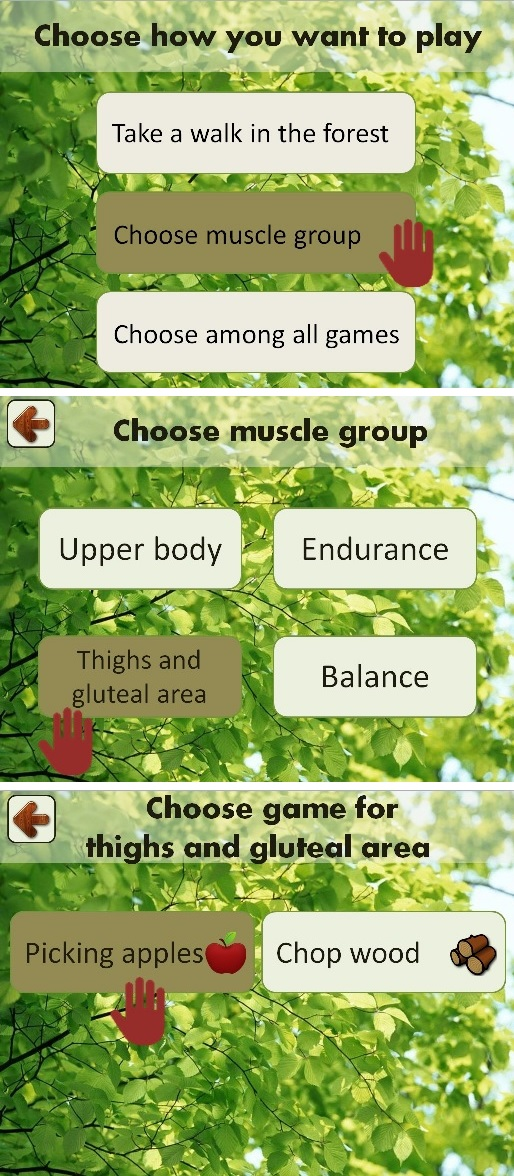
\includegraphics[scale=0.45]{menuEnglishStep1.jpg}
\caption[Menu review -  part one]{This figure shows the menu step by step, from the beginning to playing a single game, here picking apples. The selection of single games is a result of the chosen muscle group.}
\label{menu1}
\end{figure}

\begin{figure} [H]
\centering
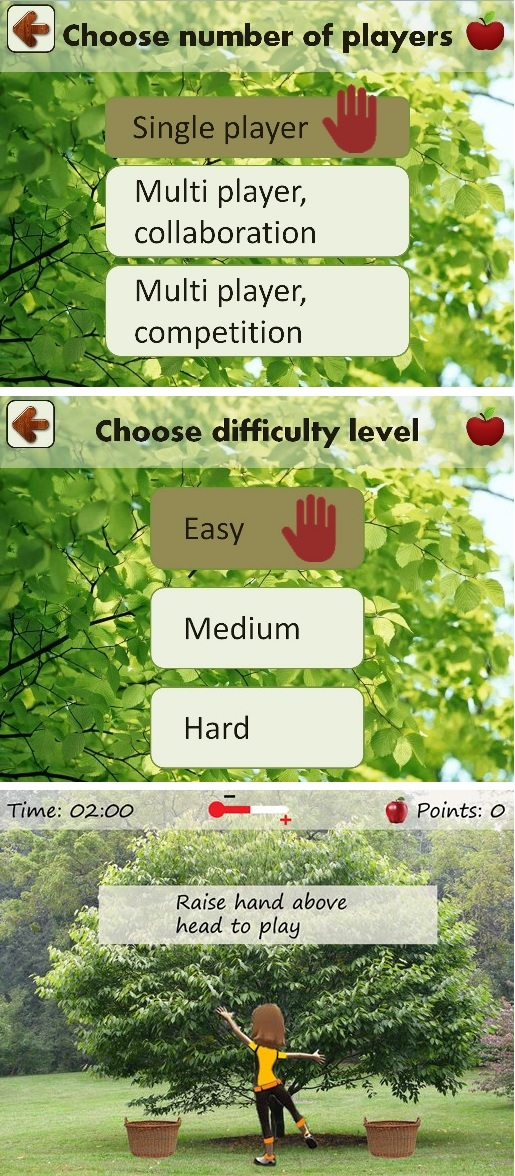
\includegraphics[scale=0.45]{menuEnglishStep2.jpg}
\caption[Menu review - part two]{This figure shows the menu step by step, from the beginning to playing a single game, here picking apples. Single player game and difficulty level easy are chosen. When ready to start the text "raise hand above head to play" is shown.}
\label{menu2}
\end{figure}

In the menu, we have used a range of green colors, and a picture of green leaves as background, to create a theme related to forest and nature. Menu buttons are arranged as list elements or in a square, depending on what is most appropriate. This is decided by the number of elements in each step, for an odd number of elements, list view will be most appropriate, while square arrangement is most suitable for an even number of elements. The size of the elements are chosen with usability in mind, there should be room for a proper font size, and it should be easy to push the right button. The buttons have a light green, almost white, background color, with a darker green outline. The text is written in black with an easy-to-read, sans serif font. The contrast between button background and text color is chosen with respect to design guideline o.14 and o.15. Taking the element's surroundings into account when choosing colors is important if you will make the element stand out. With e.g. green vegetation as surroundings, white background color, with black, dark green, or dark blue text should be chosen to create maximum contrast. This is based on guideline o.20. 

The title on each step is written in a bold, black, easy to read font, on a semi-transparent light-colored background. The title is stating what choice to be made at the current step. From the Eight Golden Rules presented in Section \ref{sec:designguide} we know that it is important to have an interface with visible information. The same rules also states that users always should be given feedback on their actions. In addition to this, there was a general opinion at workshop 1 that the informants wanted to see clearer response on their actions. We have included this in our concept by highlighting elements that are "in action", see Figure \ref{fig:avatarAction}. The player's hand movements are portrayed on the screen as an avatar hand. The avatar hand has been given a clear color and a solid fill. This has been done to avoid having the same diffuse avatar hand as in the personal trainer game.  

\begin{figure} [H]
\centering
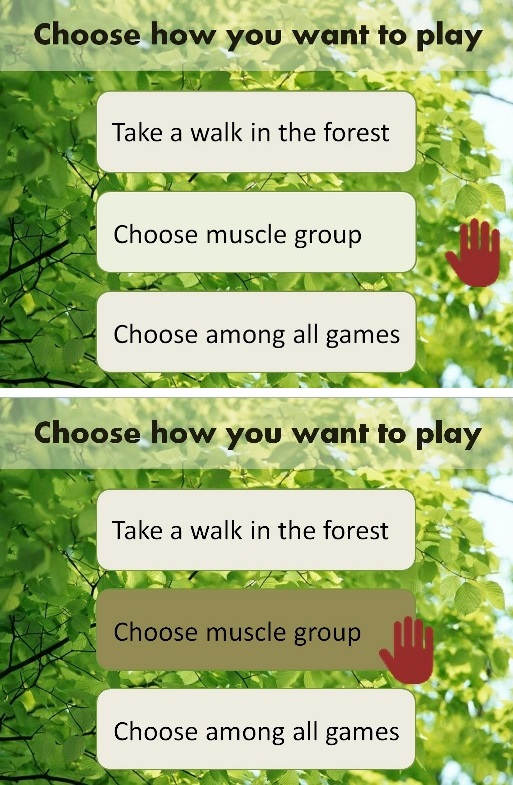
\includegraphics[scale=0.5]{menuAction.jpg}
\caption[Menu - Action and response]{In this figure an avatar hand is shown. The avatar hand will react according to the player's movements. We see that when the player move their arm over an element, it will change color.}
\label{fig:avatarAction}
\end{figure} 

Up in the left corner there is a back button, which will make it possible for users to always regret their action. The permission to reverse actions is also an important guideline from the Eight Golden Rules. The back button is shaped and colored as the other menu buttons to maintain consistency and intuitiveness. The choice of placement is based on guidelines stating that navigation should be on top, and on the natural way to read and observe information, which is from top to bottom, from left to right [KILDEee]. We avoided placing the back button in the bottom left corner to not mix it with the cancel/pause feature included in the Kinect software (holding your left hand straight 45 degrees from your body). The back button is marked with a wooden arrow, a familiar and intuitive icon related to navigation. The choice of using an wooden arrow is based on its relation to our forest theme. 

In the menu step where the player should choose between the four single games, we have used icons in addition to text on each button, see Figure \ref{fig:velgSpill}. The icons represents the challenges in each game, and they are meant to make it easier for the player to understand the game behind the button. When choosing a game, e.g. "picking apples", the icon will follow up in the right corner, to inform the player where she is headed, and to reduce memory load. This is shown in Figure \ref{fig:iconEple}.  

\begin{figure} [H]
\centering
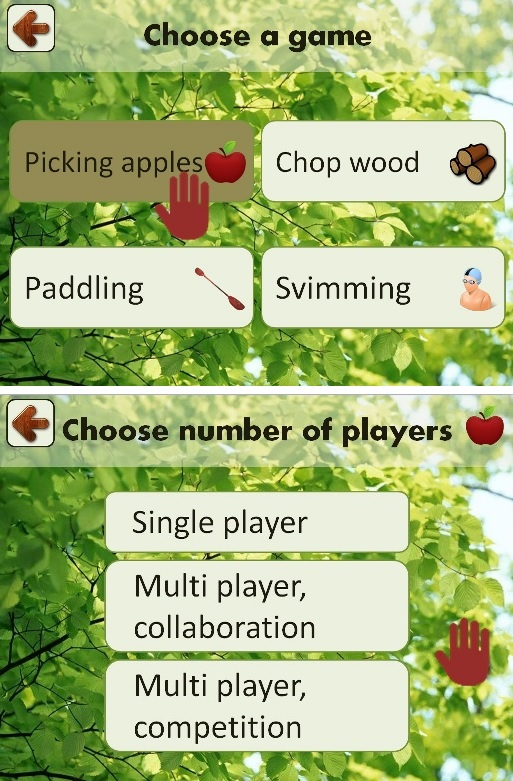
\includegraphics[scale=0.5]{menuIconApple.jpg}
\caption[Menu - use of icons]{In this figure we see that icons from menu buttons will follow the rest of the menu. Here we see that the apple icon will follow into the menu step where number of players are to be chosen.}
\label{fig:iconEple}
\end{figure} 
     
\section{A Video Game Series}
In our idea of a video game concept, our "out in the nature" exergame is a part of a video game series called "Kinect Experiences". This "Kinect Experiences" series consist of 4 individual games with the same structure as the game we have already presented. This means, one compounded game and four single games. The difference between the four video games are the main themes. In addition to "out in the nature", the "Kinect Experience" series consist of the video games "farm life", "on vacation" and "in the mountains". The five games within each video game will consist of activities that are connected to the main theme of each video game, like the exergame we already have presented. Examples of single games could be gathering eggs, and stacking hay bales in "farm life", and it could be a walk on the beach, or catching gold fish with a hoof in "on vacation". The idea behind this video game series is to offer a wide range of games, activities and exercises that fits the various interests the user group have. What this video game series would look like is shown in Figure \ref{fig:videogameseriesAlone}. 

\begin{figure} [H]
\centering
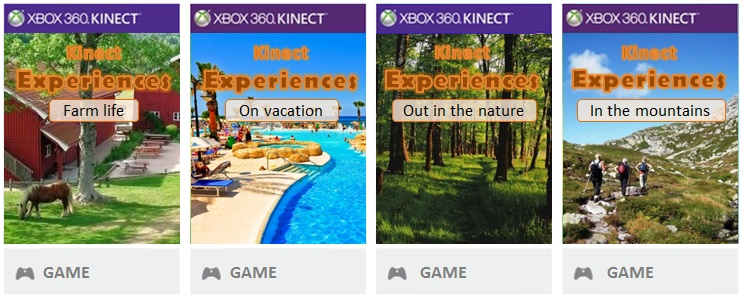
\includegraphics[scale=0.65]{videoGameSeriesAlone.jpg}
\caption[Presentation of our video game series]{A presentation of our video game series "Kinect Experiences" [modified from \cite{XboxNettside}].}
\label{fig:videogameseriesAlone}
\end{figure}

